\documentclass{article}
\usepackage{graphicx}
\usepackage{cite}
\usepackage[margin=1in]{geometry}
\usepackage[utf8]{inputenc}
\usepackage{amsmath}
\usepackage{lmodern}
\usepackage{hyperref}

\begin{document}

\title{\textbf{\Large Does our exercise affect how well we sleep? }}

\author{
    \textbf{Jonas Freeman} \\
    \textit{Harvard University} \\
    \textit{Dept. of Statistics}
    \and
    \textbf{Dries Rooryck} \\
    \textit{Harvard University} \\
    \textit{Dept. of Statistics}
    \and
    \textbf{Eva Harris} \\
    \textit{Harvard University} \\
    \textit{Dept. of Statistics}
    \and
    \textbf{Caden Woodall} \\
    \textit{Harvard University} \\
    \textit{Dept. of Statistics}
    \and
    \textbf{Sam Lindemann} \\
    \textit{Harvard University} \\
    \textit{Dept. of Statistics}
}
\date{}

\maketitle

\section{\hspace{0.5em} Introduction and Motivation}

\subsection{Motivation}

Being healthy is more than a mindset; it is a lifestyle, and people commit to this lifestyle to varying degrees. From elite athletes to the "gym-bro," everyone who takes part in this lifestyle strives for optimal results. The athletic mindset will take you far, but you will only see an impact by training the body. It is impossible to see from the outside of your body exactly what is happening internally. In the present day, even 1\% gains are celebrated achievements among professional and Olympic-level athletes. \textbf{But if you are already performing incredibly well, how do you become the best that your physiology will allow? This is where WHOOP comes in.} \\

WHOOP is one of the best fitness tracking bands in the world. All of the data is collected continuously over time, and the app interface uses extensive visuals to display this data. Its founder, Will Ahmed, is a Harvard alum who used his time at school to research the body's response to cardiovascular load and physiological strain. He believed that there was a better way to approach training geared toward maximizing performance. The band syncs roughly 100 times per second, creating a continuous dataset that provides valuable insights to allow the user to optimize their training. \cite{perlman2024} \\

In a 2016 study, the Activity Strain metric of WHOOP was proven to better predict the performance of MLB pitchers than counting the number of pitches they threw (the standard practice at the time for MLB). WHOOP's Activity Strain is a measure of the intensity and duration of physical exertion, expressed on a scale of 0 to 21. It primarily considers cardiovascular load, heart rate zones, and the duration of the activity to derive a composite score. In a piece written by Will Ahmed himself, titled "WHOOP Approved for In-Game Use in Major League Baseball," WHOOP advertises that following this study, it was the first continuous tracking device of its kind to be allowed for use in an MLB game. As an example of its application, the piece illustrated the following scenario: "Clubs could find out that Player X is no longer effective when his Day Strain hits a certain number, regardless of whether he’s thrown 50 pitches or 100 pitches to that point." \cite{ahmed2017} \\

However, there is more to predicting performance than Activity Strain. For instance, while optimizing the load on your muscles is a critical way of looking at the game, what about the recovery leading into the game? Every day, muscular structures degrade at a cellular level, and every night, they are rebuilt. This process generally occurs during restorative sleep. Restorative sleep is the combination of deep sleep (SWS) and REM sleep. Deep sleep (SWS) is known for the physical restoration that occurs throughout the body overnight. REM sleep is known as the mentally restorative stage of sleep, during which short-term memories are converted into long-term memories. \cite{whoop2023restorative}

\subsection{\hspace{0.5em} Introduction}

In this project, we will address these findings by attempting to use other athletic parameters from real WHOOP data to predict the amount of time spent in deep sleep relative to overall sleep. We hypothesize that there is a relationship between this ratio and the load that workouts (or strain) place on the body. We want to find out what the interesting relationships are that we can decompose, and we want to be able to predict consistently based on a person's exercise activity and some limited data on their sleep, what their sleep quality might look like.


\section{\hspace{0.5em} Data \& EDA}

\subsection{ \hspace{0.5em} \hspace{0.5em} Data Collection \& Cleaning}

This data was collected via the sensors on Eva's WHOOP band and synced to the WHOOP interface. We were then able to export the data in CSV format. Originally, data was provided in three categories: \textbf{Workouts.csv} (covering details like workout duration, activity type, strain, energy burned, and heart rate zones), \textbf{Sleeps.csv} (including sleep cycle durations, efficiency, debt, and consistency), and \textbf{Physiological\_Cycles.csv} (capturing recovery, resting heart rate, skin temperature, blood oxygen levels, and strain). \\

We chose to take a time-series approach. In the context of time series analysis, each day represents a single observation, allowing for the systematic tracking of workout metrics over time. We decided to create a dataframe that covered the days that Eva had a workout logged (and would be accounted for in workouts.csv), a dataframe that gathered the days that she did not have a workout logged, and then combine the two so that we have one, comprehensive dataset. There was significant redundancy in the data, which required extensive cleaning, so for simplicity, we decided to only focus on \textbf{\texttt{workouts.csv}} and \texttt{\textbf{sleeps.csv}} for this project. After cleaning, we had \textbf{one wrangled dataset} that only included data from \textbf{\texttt{workouts.csv}} and \texttt{\textbf{sleeps.csv}}. This final wrangled dataset contained 33 variables. \\

Some common issues observed were tracking errors, such as incorrect activity detection and fragmented sleep data. Fortunately, most of these errors could be corrected manually through the app before exporting the data into CSV format. 

\subsection{ {Preparing the Exploratory Variables}}

We first filtered days that included workouts based on \texttt{workouts.csv}. Columns with no data or redundant information were dropped, and the Activity.name variable was converted to a factor for categorical analysis. For clarity and interpretability, we set a floor value on the lowest number of observations of a workout. Activities labeled as "Other" (with only one observation) and "Activity" (with 65 observations) were removed. The Workout.start.time was converted to a Date type, and only the date portion was extracted to aggregate workout metrics by day. \\

Each of these daily workout summaries included several key metrics: \texttt{Total Duration}, which represents the sum of workout durations for each day, and \texttt{Total Energy Burned}, which is the total calories burned during workouts on that day. To account for workout duration when assessing heart rate, a \texttt{Weighted Average Heart Rate} was calculated, giving more weight to longer workouts. Additionally, weighted averages for each heart rate zone (1 through 5) were derived to capture the distribution of time spent in different heart rate intensities, again weighted by workout duration. By weighting the time spent in each heart rate zone by workout duration, you account for how long you maintained specific intensity levels across different workouts. This helps balance the influence of longer workouts on the daily average, which intuitively makes sense to impact the need for Deep  SWS sleep. The \texttt{Max Heart Rate} was recorded as the highest heart rate for each day, reflecting peak exertion levels. \\

To gain a comprehensive view of workout types, the dataset includes counts for each activity, where each activity type (e.g., running, cycling) is tallied based on boolean indicators (0 or 1). A new metric, \texttt{Heart Rate Zone 0}, was introduced to quantify the percentage of time spent in a resting or low-intensity state. This was calculated by subtracting the sum of the percentages of heart rate zones 1 through 5 from 100, with the result rounded to two decimal places. These daily aggregates form a robust time series dataset, facilitating the analysis of workout trends, intensity distributions, and recovery patterns over time. This structured approach to summarizing daily workout data ensures that each observation captures a comprehensive snapshot of physical activity, allowing for meaningful insights into performance and recovery. \\

The other part to time-series analysis is ensuring a complete and continuous date range. We took additional steps to ensure that this assumption was held. The process begins by generating a sequence of dates from the earliest workout date to the latest workout date in the \verb|daily_workouts| dataset. This ensures that no dates are skipped, providing a consistent timeline. \\

We then used a new dataframe to represent rest days. For each date in the range, default values are assigned to indicate no physical activity and resting heart rate conditions. Metrics like \texttt{Total Duration} and \texttt{Total Energy Burned} are set to 0, reflecting no workout activity. Heart rate-related variables, such as \texttt{Weighted Average Heart Rate} and \texttt{Max Heart Rate}, are assigned a resting value of \texttt{57 bpm}. Additionally, the weighted average heart rate zones (Zones 1 through 5) are set to 0\%, while \texttt{Heart Rate Zone 0} is set to 100\%, indicating that all heart rate activity is in the resting range. The activity count variables (e.g., Total Running, Total Cycling) are also set to 0, indicating no activity was performed on these days. By incorporating these rest days into the dataset, the continuity of the time series is maintained, which is crucial for generating accurate insights and visualizations. \\

By combining the dataframe of rest days with the original data from workouts.csv, we were able to make sure that the days with recorded workouts retain their actual metrics, such as higher maximum heart rates and real weighted heart rate zones. Our use of default placeholders in the dataframe of rest days did not overwrite or exclude higher heart rate values in the original dataset, but instead allowed for a clear distinction between workout days and rest days. After merging, the dataset was processed to remove duplicate entries, which kept only the first occurrence of a workout that was logged. To maintain the integrity of the time series, the dataset was then sorted chronologically. 

\subsection{\small {Preparing the Response Variable }}

We removed  \texttt{Cycle.start.time}, \texttt{Cycle.end.time}, \texttt{Cycle.timezone} because these are time-related metrics that are not in line with our goal. Our goal is to predict the ratio of time spent in Deep (SWS) Sleep to the overall amount of time spent asleep. We plotted a correlation matrix of sleep.csv to understand how the variables relate to one another better and to justify other changes to the dataset. In this, we found that there were four highly correlated variables. \\

\textit{Figure~\ref{fig:correlation-matrix-sleep} shows the correlation matrix for the sleep dataset.} \\

\begin{figure}[h!]
  \centering
  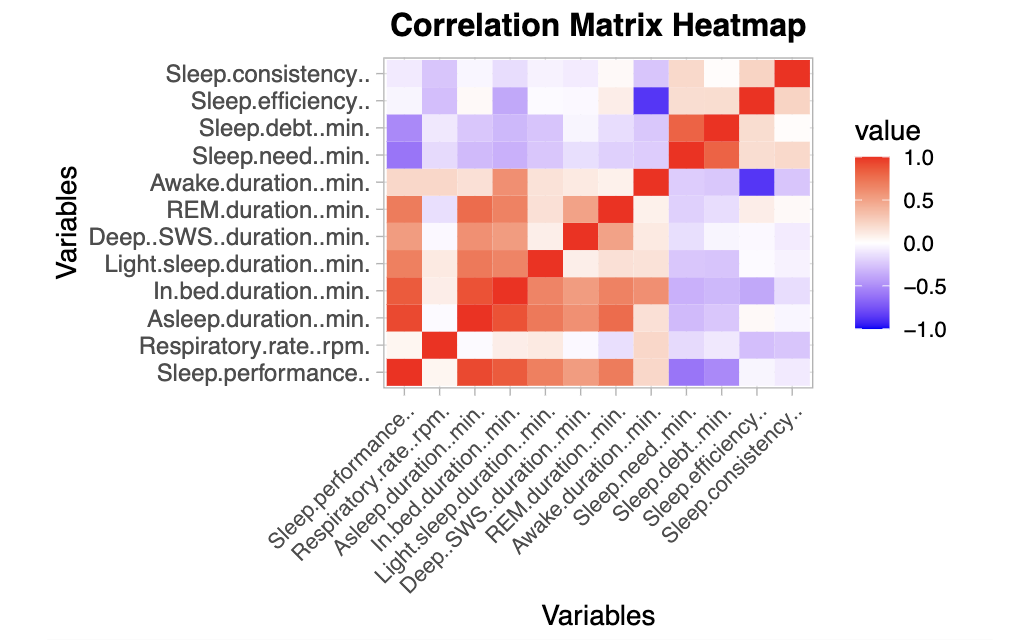
\includegraphics[width=0.7\textwidth]{images/sleepcorrelation.png}
  \caption{Correlation Matrix of the Sleep Dataset.}
  \label{fig:correlation-matrix-sleep}
\end{figure}

The correlation analysis of the sleep dataset was conducted using a threshold of 0.85 to identify highly correlated data. The resulting correlation graph revealed a strong correlation between four variable pairs: asleep duration and sleep performance, in-bed duration and sleep performance, in-bed duration and asleep duration, and sleep efficiency and awake duration. To avoid issues of collinearity, we dropped in-bed duration and sleep performance because asleep duration proved to be a reliable empirical measure. Additionally, while not caught by the threshold, sleep debt and sleep need appear to be highly correlated in the graph above. We decided to drop sleep debt as a result. \\

In-bed duration refers to the total time spent in bed, whether asleep or awake. Sleep performance is a metric calculated by a proprietary WHOOP algorithm that takes into account how well you were able to meet your body's need for sleep, incorporating sleep debt and naps. Being able to reproduce these values simply with asleep duration simplifies things significantly. Similarly, we also dropped sleep efficiency because awake duration proved to be a reliable empirical measure. Sleep efficiency is a metric calculated by a proprietary WHOOP algorithm to measure how fast you go to sleep. \\

Nap statistics were then calculated by converting \texttt{Wake.onset} to \texttt{Wake.date} (date-only format) and grouping by \texttt{Wake.date}. For each date, \texttt{Nap.count} was computed as the number of distinct wake-up times minus one, and \texttt{Nap.duration} was the total sleep duration minus the longest sleep (main sleep). If no naps occurred, \texttt{Nap.duration} was set to zero. This provided clear daily measures of nap frequency and duration. \\

The main sleep session for each day was identified as the entry with the maximum \texttt{Asleep.duration..min.}, retaining the first occurrence in case of ties. To align sleep with workout data, a \texttt{Sleep.date} column was created by subtracting one day from \texttt{Wake.onset}, reflecting the night the user went to sleep. The main sleep data was merged with nap data using a left join on \texttt{Sleep.date} and \texttt{Wake.date}, filtering out rows with missing nap statistics. The sleep data was grouped by the wake-up date to organize sleep data by the day the user woke up. The final version of \textbf{Sleeps.csv} contained primary metrics for sleep duration, nap count, and total nap duration, and all aligned by date for consistency with the cleaned \textbf{Workouts.csv} data. 

\subsection{\small {Combining Exploratory and Response Data}}

Next, we used the date of each observation to perform an inner join that combines the dataset that contained our exploratory variables with the dataset that contained our response variables. Additionally, to streamline this dataset, time-related columns such as \verb|Sleep.onset|, \verb|Wake.onset|, and \verb|as.Date(Wake.onset)| were removed, as well as the count for each type of workout. The number of times Eva logged each type of workout is extraneous because it is the heart rate zones that trains the cardiovascular system, irrespective of the actual exercise or method used to achieve this heart rate. 

\subsection{\small{Our final wrangled dataset}}

The final dataset included the following columns: Respiratory rate (rpm), asleep duration (min), light sleep duration (min), deep SWS duration (min), REM duration (min), awake duration (min), sleep need (min), sleep consistency, nap count, nap duration, total duration (min), total energy burned (cal), weighted average heart rate (HR), weighted average HR zone 1, weighted average HR zone 2, weighted average HR zone 3, weighted average HR zone 4, weighted average HR zone 5, maximum HR (bpm), and weighted average HR zone 0. The following correlation matrix demonstrates how these variables relate to eachother within the final dataset. \\

\textit{Figure~\ref{fig:correlation-matrix-cleaned} shows the correlation matrix for the cleaned dataset.}

\begin{figure}[h!]
  \centering
  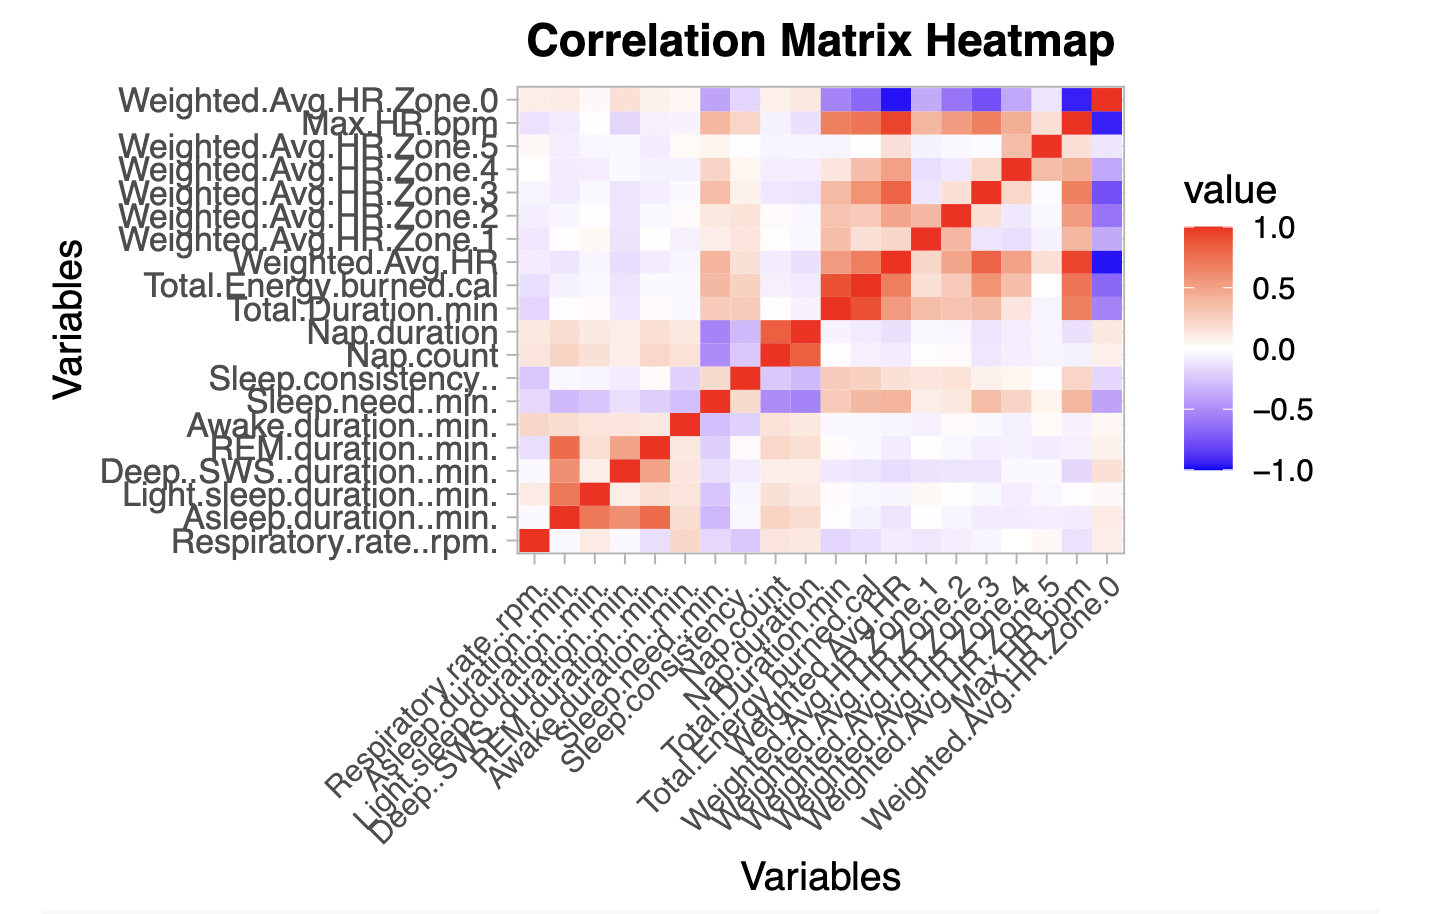
\includegraphics[width=0.7\textwidth]{images/cleanedcorrelation.png}
  \caption{Correlation Matrix of the Cleaned Dataset.}
  \label{fig:correlation-matrix-cleaned}
\end{figure}

\newpage

\subsection{ \hspace{0.5em} \hspace{0.5em} EDA \& Hypothesis}

We initially hypothesized that \textbf{WHOOP's Activity Strain} (Activity Strain) would be the parameter with the biggest impact on the ratio of Deep (SWS) sleep to the total mount of sleep. However, after further thought we realized that the metric was likely a functin of data we already have. To examine this, we decided to use Activity Strain as the focus for our exploratory data analysis. In this EDA, we tested whether we needed Activity Strain to experiment with Deep SWS Sleep. The algorithm WHOOP uses to calculate Activity Strain is proprietary, but if other data could be used to strongly predict this measure then the metric would be collinear. In which case, it would be best to drop the metric entirely in an effort to avoid redundancy. In the next part of our EDA we attempted to model WHOOP's Activity strain via a linear regression. \\

To predict \textbf{WHOOP's Activity Strain}, we created a regression that had Activity Strain as our a dependent variable. Because our goal was to test the redundancy of including this metric, we used all variables that were not distance-related or time-related as our exploratory variables. This meant excluding GPS.enabled, Distance..meters., Altitude.gain..meters., Altitude.change..meters., Cycle.start.time, Cycle.end.time, Cycle.timezone, Workout.start.time, Workout.end.time, and Activity.name. \\

\bigskip

\textbf{Linear Regression Model for Activity Strain}

\begin{equation}
\text{Activity Strain} \sim 
\left(
\begin{split}
\text{Heart Rate Avg (bpm)} + \text{Heart Rate Max (bpm)} + \text{Duration (min)} + \\
\text{Total Energy Burned (cal)} + \text{Weighted Avg HR} + \text{HR Zone 0} + \text{HR Zone 1} + \\
\text{HR Zone 2} + \text{HR Zone 3} + \text{HR Zone 4} + \text{HR Zone 5}
\end{split}
\right)
\end{equation}
\bigskip

This high level of explanatory power suggested that the simplified model captures the essential predictors, such as heart rate data (max heart rate, average heart rate, and heart rate zones) and workout duration. We then decided to check the observe the correlation matrix for of the workouts dataset for further insight about how our predictors relate to one another. \\

\textit{Figure~\ref{fig:correlation-matrix-workouts} shows the correlation matrix for the workouts dataset.} \\

\begin{figure}[h!]
  \centering
  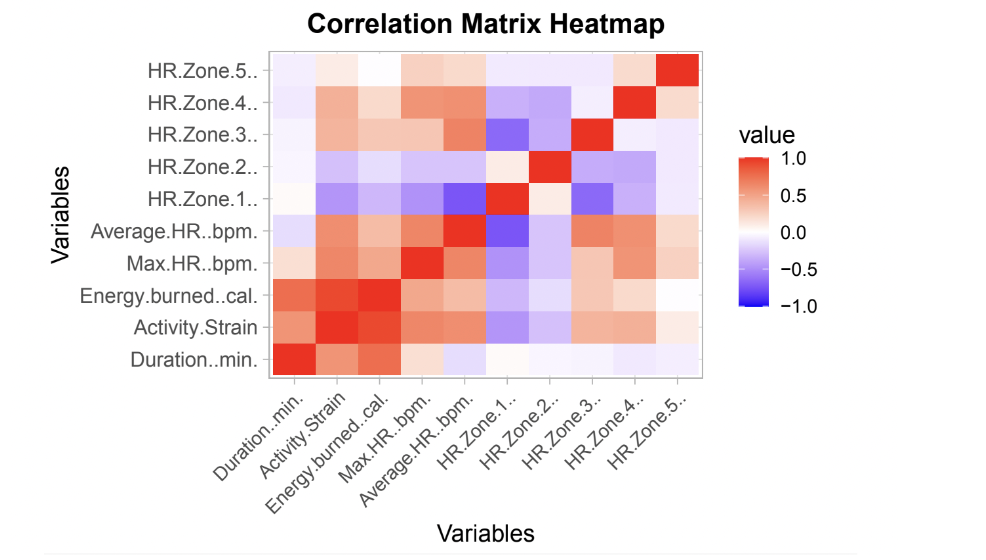
\includegraphics[width=0.7\textwidth]{images/workoutscorrelation.png}
  \caption{Correlation Matrix of the Workouts Dataset.}
  \label{fig:correlation-matrix-workouts}
\end{figure}

The correlation analysis of the workouts dataset was conducted using a threshold of $0.85$ to identify highly correlated data. The resulting correlation graph revealed a strong correlation between Activity Strain and Energy Burned. To avoid issues of collinearity, the Activity Strain column was dropped, as Energy Burned serves as a reliable empirical measure of physical exertion. These changes were reflected in our final dataset. \\

\section{\hspace{0.5em} Methods and Results}

\subsection{\hspace{0.5em} Methods for Inference Model}

The baseline model was a generalized linear regression on the ratio of deep sleep to overall sleep across different days. \\

This regression relied on a comprehensive set of variables that included respiratory rate (\verb|Respiratory.rate..rpm.|), total sleep duration (\verb|Asleep.duration..min.|), deep sleep duration (\verb|Deep..SWS..duration..min.|), nap count (\verb|Nap.count|),  nap duration (\verb|Nap.duration|), total workout duration (\verb|Total.Duration.min.|)  total energy burned (\verb|Total.Energy.burned.cal|),  and heart rate data including the weighted average heart rate (\verb|Weighted.Avg.HR|), weighted heart rate zone distributions (\verb|Weighted.Avg.HR.Zone.0| through \verb|Weighted.Avg.HR.Zone.5|) and maximum heart rate (\verb|Max.HR.bpm|). There were no interaction terms. The aim for this diversity was to provide a comprehensive basis for predicting the ratio of deep sleep.
 
\subsubsection{\hspace{0.5em} Assumptions for Baseline Model}

There are a few things that must hold for linear regression to work here for inference. First, for linear regression we require that the response is continuous. The ratio we are trying to predict is continuous, but it is a fraction out of 1. But taking that into account would be out of the scope of this class. The second assumption is that the predictors are not highly correlated, and we can tell they are not from a correlation matrix from our EDA. Last, we first checked the standard assumptions: Existence, Linearity, Independence, and Homoscedasticity (ELIH). The results of these checks are visualized through residual diagnostics, including Residuals vs. Fitted plots, Q-Q plots of residuals, and histograms.

\begin{itemize}
    \item \textbf{Linearity and Homoscedasticity:}  
    The Residuals vs. Fitted plot (Figure~\ref{fig:residuals-fitted}) shows that the residuals are largely centered around zero with no clear non-linear pattern. However, there is slight heteroscedasticity, as evidenced by uneven spread near the center of the fitted values.

    \item \textbf{Normality of Residuals:}  
    The Q-Q plot (Figure~\ref{fig:qq-residuals}) indicates that the residuals follow an approximately normal distribution, with minor deviations in the tails caused by a few outliers.

    \item \textbf{Independence of Residuals:}  
    The Residuals vs. Total Duration plot (Figure~\ref{fig:residuals-duration}) demonstrates that residuals are randomly scattered, suggesting no relationship between the residuals and predictor values.

    \item \textbf{Residual Distribution:}  
    The histogram of residuals (Figure~\ref{fig:hist-residuals}) shows a roughly bell-shaped curve, supporting the assumption of normally distributed errors.

\end{itemize}

\begin{figure}[h!]
  \centering
  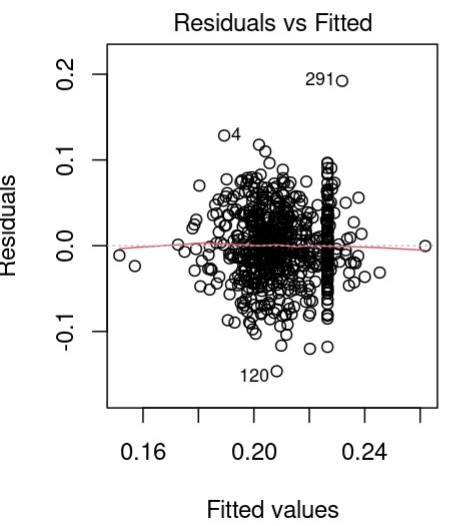
\includegraphics[width=0.4\textwidth]{images/residuals_vs_fitted.png}
  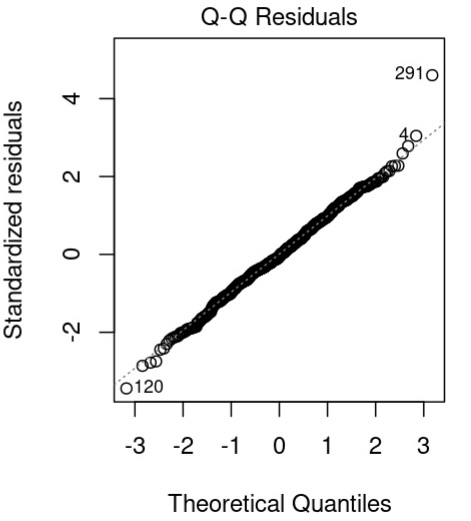
\includegraphics[width=0.4\textwidth]{images/qq_residuals.png}
  \caption{Residuals vs. Fitted (left) and Q-Q Plot of Residuals (right).}
  \label{fig:residuals-fitted}
  \label{fig:qq-residuals}
\end{figure}

\begin{figure}[h!]
  \centering
  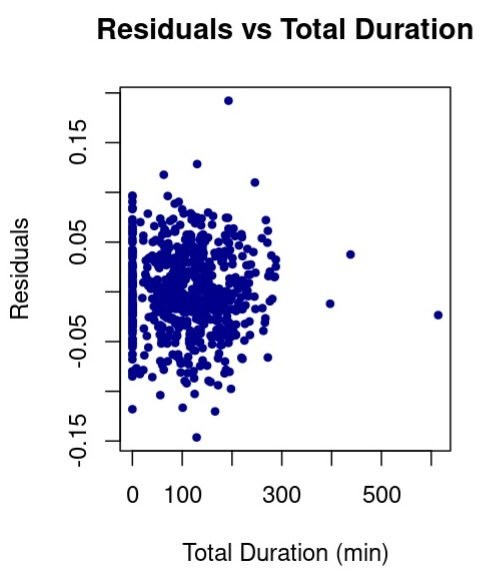
\includegraphics[width=0.4\textwidth]{images/residuals_vs_duration.png}
  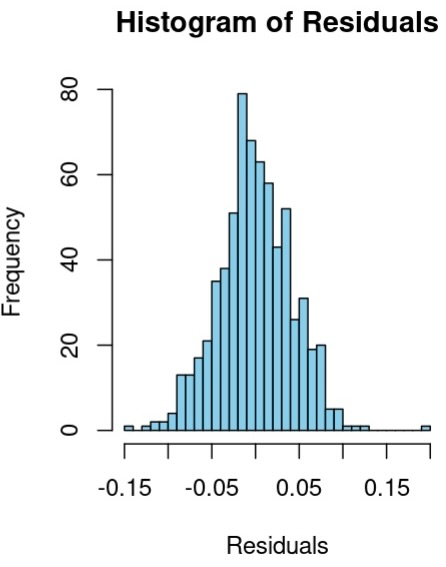
\includegraphics[width=0.4\textwidth]{images/histogram_residuals.png}
  \caption{Residuals vs. Total Duration (left) and Histogram of Residuals (right).}
  \label{fig:residuals-duration}
  \label{fig:hist-residuals}
\end{figure}

The residual diagnostics confirm that the assumptions of linearity, independence, and normality are approximately satisfied. Minor deviations in homoscedasticity and the presence of a few outliers should be addressed in future models through transformations or robust regression techniques.

\subsubsection{ \hspace{0.5em} Results for more Sophisticated Models}

We implemented one baseline model and two sophisticated models for inference in our analysis. The baseline model was a the most basic version of a linear regression designed to predict the ratio of SWS (Deep) sleep to overall sleep using the given parameters. The parameters of the model are Respiratory Rate (rpm), Light Sleep Duration (min), REM Duration (min), Awake Duration (min), Sleep Need (min), Sleep Consistency, Nap Count, Nap Duration, Total Duration (min), Total Energy Burned (cal), Weighted Avg HR, HR Zone 1, HR Zone 2, HR Zone 3, HR Zone 4, HR Zone 5, Max HR (bpm), and HR Zone 0. It had no interaction terms. The \textbf{adjusted $R^2$ value }of the baseline model was \textbf{$0.347$.} \\

Our \textbf{first attempt} at a more sophisticated model included an interaction term with \verb|Total.Energy.burned.cal|. This variable captures the total calories burned during the day, and is often reflects the total physiological load of the day. In the code file, this model is \verb|model_rr|.The model uses all predictors in the dataset (like our baseline model) but builds on this model by including an interaction using the total energy burned during the day. Like the baseline model, the response variable is \(\text{Deep..SWS..duration..min. / Asleep.duration..min.}\), which represents the proportion of sleep spent in deep sleep. 
The \textbf{adjusted \(R^2\)} value of the interaction effects this model was \(0.351\), which is significantly higher than our baseline model (\(0.347\)). \\

By including the interactive term, the model is able to capture both the direct effect of total energy burned on the deep sleep ratio and its interactions with every other variable in the dataset. These interactions allow the model to evaluate how the relationship between each predictor and the deep sleep ratio changes based on the total energy burned. For instance, we theorized that the influence of variables such as average heart rate or nap duration on deep sleep may vary depending on the amount of energy expended during the day. \\

With our \textbf{second attempt} at a more sophisticated model, we developed a linear regression that predicts the deep sleep ratio by incorporating all main effects and two-way interactions between the predictors. In the code file, this model is \verb|model_full|. While this approach captures more intricate relationships, it also introduces risks such as overfitting and reduced interpretability due to the interaction terms. In particular, we may have created high collinearity among predictors. The \textbf{adjusted $R^2$  value }for this model is \textbf{$0.364$}. \\

Given the adjusted $R^2$ values and overall complexity, it makes sense that the more sophisticated models would be suitable candidates for backward stepwise selection. Backward step selection systematically simplifies the model by eliminating the insignificant interaction terms. To evaluate the quality of the models at each step of this process, we employed the Akaike Information Criterion (AIC), which assesses model performance relative to other potential models. \\

Originally when we ran these models, we had a higher adjusted $R^2$ value in the interaction model. Even though adjusted $R^2$ adjusts for the total number of parameters used, this outcome didn't seem likely. After this, we re-examined our code and made corrections. However, to ensure that we would conclude with the most optimal model we could find, we decided to conduct the stepwise selection process twice: once using each more-sophisticated model. The first more-sophisticated model yielded an AIC of \textbf{-4415.95}, which is notably lower than the AIC of \textbf{-4295.39} obtained for the second more-sophisticated model. Below is a representation of the models that resulted when backward selection was applied to each more-sophisticated model.

\newpage

\textbf{Backward Selction, First More-Sophisticated Model: $\frac{\text{Deep SWS Duration (min)}}{\text{Asleep Duration (min)}}$}

\[
\sim \text{Total Energy Burned (cal)} \times
\]

\begin{equation}
\left(
\begin{split}
\text{Respiratory Rate (rpm)} + \text{Light Sleep Duration (min)} + \text{REM Duration (min)} + \text{Awake Duration (min)} + \\
\text{Sleep Need (min)} + \text{Sleep Consistency} + \text{Nap Count} + \text{Nap Duration} + \\
\text{Total Duration (min)} + \text{Total Energy Burned (cal)} + \text{Weighted Avg HR} + \text{HR Zone 1} + \\
\text{HR Zone 2} + \text{HR Zone 3} + \text{HR Zone 4} + \text{HR Zone 5} + \text{Max HR (bpm)} + \text{HR Zone 0}
\end{split}
\right)
\end{equation}


\bigskip

\textbf{Backward Selection, Second More-Sophisticated Model: $\frac{\text{Deep SWS Duration (min)}}{\text{Asleep Duration (min)}}$}

\begin{equation}
\sim 
\left(
\begin{split}
\text{Respiratory Rate (rpm)} + \text{Light Sleep Duration (min)} + \text{REM Duration (min)} + \text{Awake Duration (min)} + \\
\text{Sleep Need (min)} + \text{Sleep Consistency} + \\
\text{Nap Count} + \text{Nap Duration} + \text{Total Duration (min)} + \\
\text{Total Energy Burned (cal)} + \text{Weighted Avg HR} + \text{HR Zone 1} + \\
\text{HR Zone 2} + \text{HR Zone 3} + \text{HR Zone 4} + \text{HR Zone 5} + \\
\text{Max HR (bpm)} + \text{HR Zone 0}
\end{split}
\right)^2
\end{equation}

\bigskip
\bigskip

Backward selection is a stepwise regression technique that begins with the most complex model. This means including all predictors. At each step, it evaluates the impact of removing one predictor using a metric such as AIC, and the least significant predictor is removed. This process is repeated until removing any further predictors would reduce the model's performance. Therefore, as a whole, this method helps to simplify models while retaining only the most significant predictors. Given this logic, it makes sense that by using this method, our second more-sophisticated model was able to reach the best adjusted $R^2$ so far.\\

\begin{table}[h!]
\centering
\caption{Adjusted \(R^2\) Values for Different Models}
\label{tab:adjusted-r2-models}
\begin{tabular}{|l|c|}
\hline
\textbf{Model}                                                   & \textbf{Adjusted \(R^2\)} \\ \hline
Baseline Model                                                   & 0.347                     \\ \hline
First Sophisticated Model                                        & 0.351                     \\ \hline
Second Sophisticated Model                                               & 0.364                     \\ \hline
Backward Stepwise (First Sophisticated Model)                   & 0.363                     \\ \hline
Forward Stepwise (First Sophisticated Model)                    & 0.353    \\ \hline
Backward Stepwise (Second Sophisticated Model)                   & 0.419                     \\ \hline
Forward Stepwise (Second Sophisticated  Model)                    & 0.367    
    \\ \hline

\end{tabular}
\end{table}

\bigskip

Given this table, we came to the following conclusions. In both models, backward selection produced a higher adjusted $R^2$ value. Through step selection, the first more-sophisticated model improved from $0.351$ to $0.363$ and the second more-sophisticated model improved from $0.364$ to $0.419$. It should be noted that in both models, backward selection had a higher adjusted $R^2$ value than forward selection. The adjusted $R^2$ for the most optimal model was $0.419$, which makes sense given that backward selection is designed to start from a highly complex model. This makes sense because backward selection is designed to start with the most complex model, and our second more-sophisticated model was more complex than any other model we have dealt with so far in this piece. \\

One potential hazard to be wary of is that interaction terms may exacerbate multicollinearity issues, especially if the predictors involved in the interaction are correlated. It is important to note that high multicollinearity can lead to inflated standard errors and less accurate coefficient estimates. \\

\textit{Please see \textbf{Appendix} for the fitted/residuals plots and QQ plots for each of the odels referenced in this section.}

\subsection{Inference on significant predictors}

For our baseline model that explains a decent amount of the variance in the response, we also relay what we found from linear regression to be significant predictors at the 0.05-level. \\


\begin{table}[h!]
\centering
\caption{Baseline Model Outputs from \texttt{lm}.}
\begin{tabular}{lcccc}
\hline
\textbf{Predictor}              & \textbf{Estimate}   & \textbf{Std. Error} & \textbf{t Value} & \textbf{p-Value} \\ \hline
Intercept                       & -30.97              & 75.89               & -0.408           & 0.6834           \\
Respiratory Rate (rpm)          & 0.00001098          & 0.002646            & 0.004            & 0.9967           \\
Light Sleep Duration (min)      & -0.0005288          & 0.00003224          & -16.399          & $<2 \times 10^{-16}***$ \\
REM Duration (min)              & -0.00006081         & 0.00003578          & -1.700           & 0.0897\textsuperscript{.} \\
Awake Duration (min)            & 0.0000865           & 0.00004466          & 1.937            & 0.0532\textsuperscript{.} \\
Sleep Need (min)                & 0.00003521          & 0.00004005          & 0.879            & 0.3796           \\
Sleep Consistency               & -0.0002069          & 0.0001093           & -1.893           & 0.0588\textsuperscript{.} \\
Nap Count                       & -0.004514           & 0.007226            & -0.625           & 0.5324           \\
Nap Duration                    & 0.00005424          & 0.0001443           & 0.376            & 0.7071           \\
Total Duration (min)            & 0.00008922          & 0.00007057          & 1.264            & 0.2066           \\
Total Energy Burned (cal)       & -0.00001293         & 0.00001236          & -1.046           & 0.2958           \\
Weighted Avg HR                 & 0.000444           & 0.0004750           & 0.935            & 0.3503           \\
Weighted Avg HR Zone 1          & 0.3125              & 0.7590              & 0.412            & 0.6807           \\
Weighted Avg HR Zone 2          & 0.3126              & 0.7590              & 0.412            & 0.6805           \\
Weighted Avg HR Zone 3          & 0.3126              & 0.7590              & 0.412            & 0.6806           \\
Weighted Avg HR Zone 4          & 0.3128              & 0.7590              & 0.412            & 0.6804           \\
Weighted Avg HR Zone 5          & 0.3130              & 0.7590              & 0.412            & 0.6802           \\
Max HR (bpm)                    & -0.0003551          & 0.0001559           & -2.278           & 0.0230\textsuperscript{*} \\
Weighted Avg HR Zone 0          & 0.3127              & 0.7590              & 0.412            & 0.6805           \\ \hline
\end{tabular}
\label{tab:baseline_model_outputs}
\end{table}



The duration of light sleep, the number of hours awake, the WHOOP-calculated sleep needed, and the duration of naps during the day (0 when there are no naps) were all statistically significant predictors. Perhaps unsurprisingly, in a basic model with no interaction terms, the predictors that were most important to predict the ratio of deep sleep to total sleep were all sleep-related, not exercise-related. Intuitively, it makes sense that one could explain the proportion of deep sleep by using the light sleep duration as an inverse correlative variable. \\

Likewise, to calculate their metric for sleep-need, WHOOP uses a combination of the person’s baseline sleep need (generally 7.6 hours), physical exertion through the day (strain), previous sleep debt, and naps. Additionally, it would also make sense for that person to have more time spent in Deep (SWS) sleep. \cite{whoop_sleep}\cite{whoop_sleep_debt} \\

Our best model had too many predictors to fully analyze its output in this piece, however, we included a table of significant predictors and their respective p-values. While there were many more interaction terms, there were also more variables were statistically significant in this model that related to exercise. To give a couple examples, this included the interaction between the total energy burnt and the weighted average heartrate. The complete table of the significant predictors from our best model (and their varying levels of significance) is below.

\begin{table}[h!]
\centering
\caption{Significant Coefficients and Levels of Significance}
\begin{tabular}{lcccc}
\hline
\textbf{Predictor} & \textbf{Estimate} & \textbf{Std. Error} & \textbf{\(p\)-value} & \textbf{Significance Level} \\ \hline
Respiratory.rate..rpm.:Awake.duration..min.   & -2.459e-04 & 1.083e-04 & 0.023642 & * \\
Light.sleep.duration..min.:Sleep.consistency.. & -8.457e-06 & 2.910e-06 & 0.003823 & ** \\
Total.Energy.burned.cal:Weighted.Avg.HR        & 1.987e-05  & 5.936e-06 & 0.000881 & *** \\
Weighted.Avg.HR.Zone.1:Weighted.Avg.HR.Zone.4 & -2.408e-04 & 1.103e-04 & 0.029573 & * \\
Weighted.Avg.HR.Zone.2:Weighted.Avg.HR.Zone.3 & -6.505e-05 & 2.810e-05 & 0.021019 & * \\
Weighted.Avg.HR.Zone.3:Weighted.Avg.HR.Zone.0 & -1.624e-04 & 7.313e-05 & 0.026864 & * \\
\hline
\end{tabular}
\label{tab:significant_coefficients_with_pvalues}
\end{table}

\subsection{ \hspace{0.5em} Methods for Prediction Models}

Our approach to try and do prediction will use a different response variable for what we are trying to capture: \textit{a good nights' sleep}, which is still related to the ratio of deep-sleep to total sleep. We will instead classify days into good-sleeps and bad-sleeps. It seemed like the median of days had a deep-sleep-ratio of 0.211. so we added a binary response variable that is 1 for all sleeps with this variable above 0.211 (n=235), and 0 for sleeps with the variable below 0.5 (n=236). Using a binary response will allow us to evaluate the results of our prediction more meaningfully, as a mean-squared error of prediction on a response that is a number between 0 and 1 is not sensible. Binary prediction is still quite useful as the core question we are trying to get at is whether we can predict whether someone will have good quality sleep based on their exercise patterns.

\begin{figure}[h!]
  \centering
  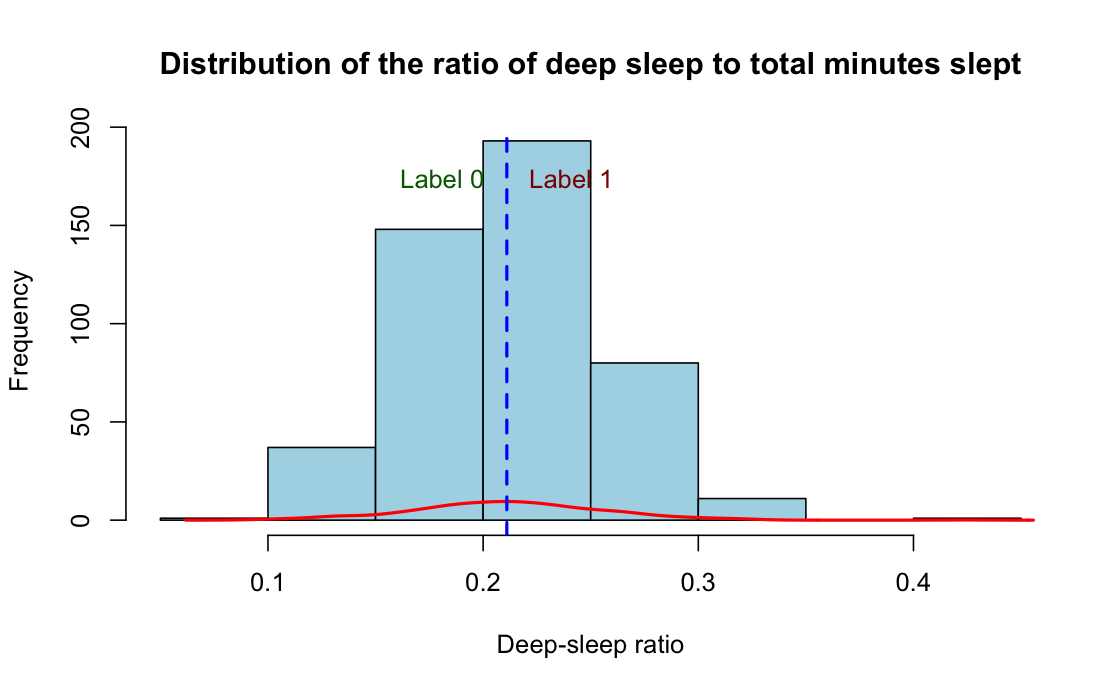
\includegraphics[width=0.6\textwidth]{images/000020.png}
  \caption{Histogram for the distribution of deep sleep.}
  \label{fig:correlation-matrix-cleaned}
\end{figure}

\subsubsection{\hspace{0.5em} Data Splitting \& Model Evaluation}
Across the observations (days), We used a seed of 139 to maintain reproducibility across the different predictive models we tried. Across all days, we randomly split 80 percent of our data into the training set and 20 percent into the testing set. Our dataset is reasonably balanced, so accuracy should be a good metric of our binary predictors' performance, but we have also included the metrics of precision, recall, and F1-score, the harmonic mean of precision and recall.
\subsubsection{ \hspace{0.5em} Baseline Predictive Linear Model}

We use a simple logistic regression model from the \texttt{glm} package with the binomial family. If the classifier predicts a probability of greater than 0.5 for a sleep on that day, based on the characteristics of the exercise done that day, of being classified as a good sleep, then the model will classify it as a good-sleep day. The assumptions of logistic regression hold here: we are predicting a binary variable, we have a large enough sample size (n=471), and we have little multicolinearity among our predictors.





\subsubsection{\hspace{0.5em} Additions to logistic regression}

We experimented with the following models with the following settings for binary prediction:
\begin{enumerate}
    \item LASSO regression: to shrink coefficients with less predictive power, to prevent overfitting. We tune the regularization parameter $\lambda$ using cross-validation.
    \item k-nearest neighbors: predicting the label based on the majority class of the $k$ nearest data points seen in training. We tune the hyperparameter $k$ by cross-validating over 10 values of $k.$
    \item Random Forest: Used to test efficacy of tree-based against the linear methods we focus on in this class. We used cross-validation to set \texttt{mtry,} the number of predictors selected for consideration at each split.
    \item Gradient-Boosted Trees: Also as a point of comparison against linear models, we use cross-validation to select nrounds and the maximum depth of each tree in the ensemble.
    \item Support Vector Machines. We tune cost of misclassification and RBF kernel width by cross-validation.
\end{enumerate}

\subsubsection{\hspace{0.5em} Prediction Results}

\begin{table}[h!]
\centering
\caption{Model Performance Metrics on the Test Set}
\begin{tabular}{lcccc}
\hline
\textbf{Model} & \textbf{Precision} & \textbf{Accuracy} & \textbf{Recall} & \textbf{F1} \\
\hline
Logistic Regression (Baseline)   & 0.573 & 0.639 & 0.729 & 0.642 \\
Logistic Regression w/ LASSO     & 0.581 & 0.647 & 0.729 & 0.647 \\
K-Nearest-Neighbors              & 0.551 & 0.617 & 0.729 & 0.628 \\
Random Forest                    & 0.556 & 0.617 & 0.678 & 0.611 \\
Gradient-Boosted Trees           & 0.589 & 0.654 & 0.729 & 0.652 \\
Support Vector Machines          & 0.577 & 0.647 & 0.763 & 0.657 \\
\hline
\end{tabular}
\label{tab:model_performance}
\end{table}



We present a table of the performance on the hold-out test set of accuracy, precision, recall and F1-score, for the 6 models we fit. As we can tell, the models all have 60-plus percent accuracy and F-1 score. Interestingly, the tree-based methods do not present a significant advantage over the linear models here. All models perform in the same ballpark, with gradient-boosting providing a small edge in terms of accuracy and F-1. All models perform slightly better than the naive baseline of 50\% accuracy.\\

\begin{figure}[h!]
\centering
\fbox{%
\begin{minipage}{0.48\textwidth}
    \centering
    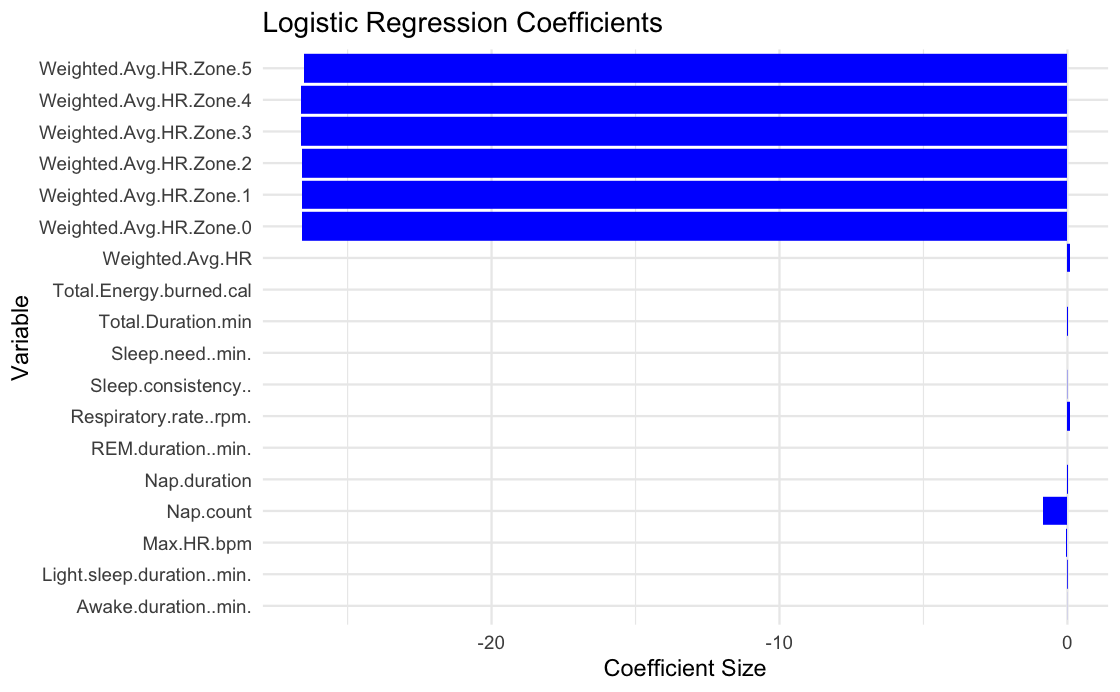
\includegraphics[width=\textwidth]{images/000070.png}

\end{minipage}
\hfill
\begin{minipage}{0.48\textwidth}
    \centering
    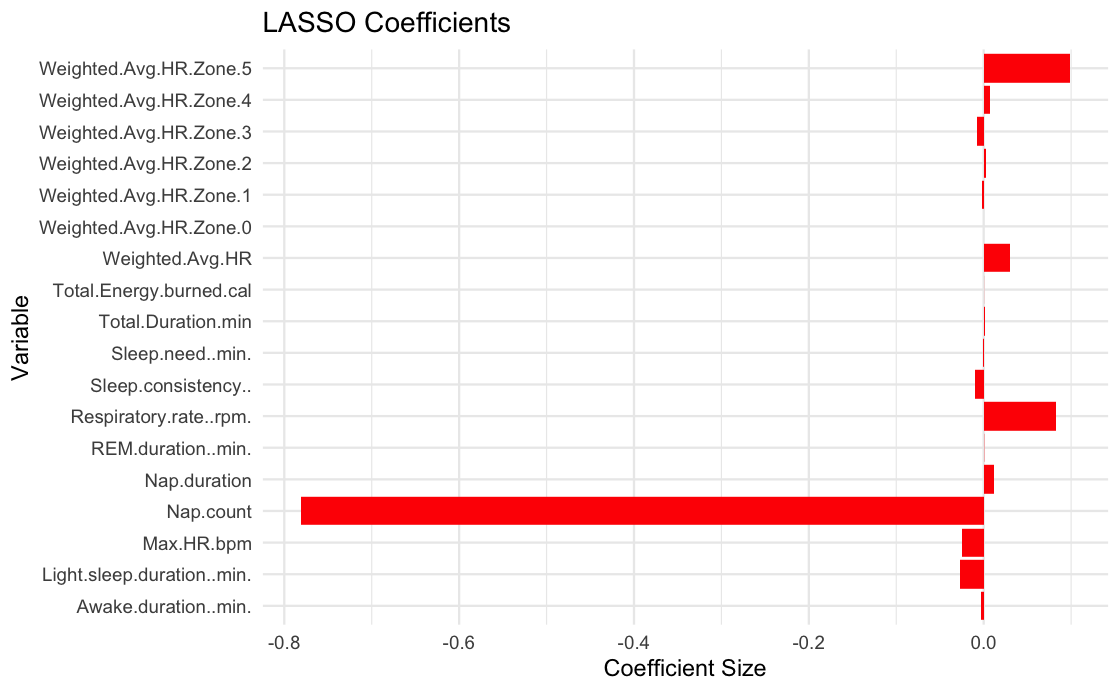
\includegraphics[width=\textwidth]{images/000071.png}

\end{minipage}
}
\caption{Comparison of Absolute Coefficient Sizes: Logistic vs LASSO Regression.}
\label{fig:coeff_comparison}
\end{figure}

We have plotted the relative sizes of the coefficients for each model separately in the below two charts. We see that LASSO shrunk the variables \texttt{Weighted.Avg.HR.Zone.0}, and \texttt{ Total Energy Burned } to zero. Interestingly, LASSO assigns a high relative importance to the number of naps taken during the day to predict the quality of sleep.

\section{\hspace{0.5em} Conclusion and Further Work}

We conclude that some of the quality of an individual's sleep can be measured from their exercise patterns, especially from the perspective of binary prediction on whether someone slept well. We did find certain statistically significant associations though between exercise patterns and one's sleep. One area of further research would be to find a great metric for the quality of one's sleep. Another interesting experiment could be to include more binary data, based on the type of exercise done during the day, for example, to see if that affects the relationship between predictor and response. \\

Ultimately, a number of improvements could be made in the future that would continue our research. Firstly, collecting predictive variables closer to the time of one's sleep may ultimately prove more useful in pure prediction of sleep quality. Furthermore, the relatively small size of our dataset in terms of observations and the fact that we are limited to the data of one individual means that our prediction method will likely not generalize well to the population, and is perhaps not even robust to the sleep Eva is likely to have one year from now. Also, we should properly limit ourselves to strictly data from exercise-related activity.\\

Still though, our work suggests that some insights can be gained for improving sleep quality based on what is done during the day. We saw for example, surprisingly, that one's overall weighted average heart-rate zone is statistically significant and positively correlated with the ratio of deep sleep to total sleep. \\
\newpage

\bibliographystyle{plain}  
\bibliography{references}

\newpage


\section{Appendix: Parameter Distributions \& Model Plots}

A GitHub page with all of our experiments and data for replication can be found at \href{https://github.com/drooryck/whoop-sleep}{our GitHub Repository}


\begin{figure}[h!]
  \centering
  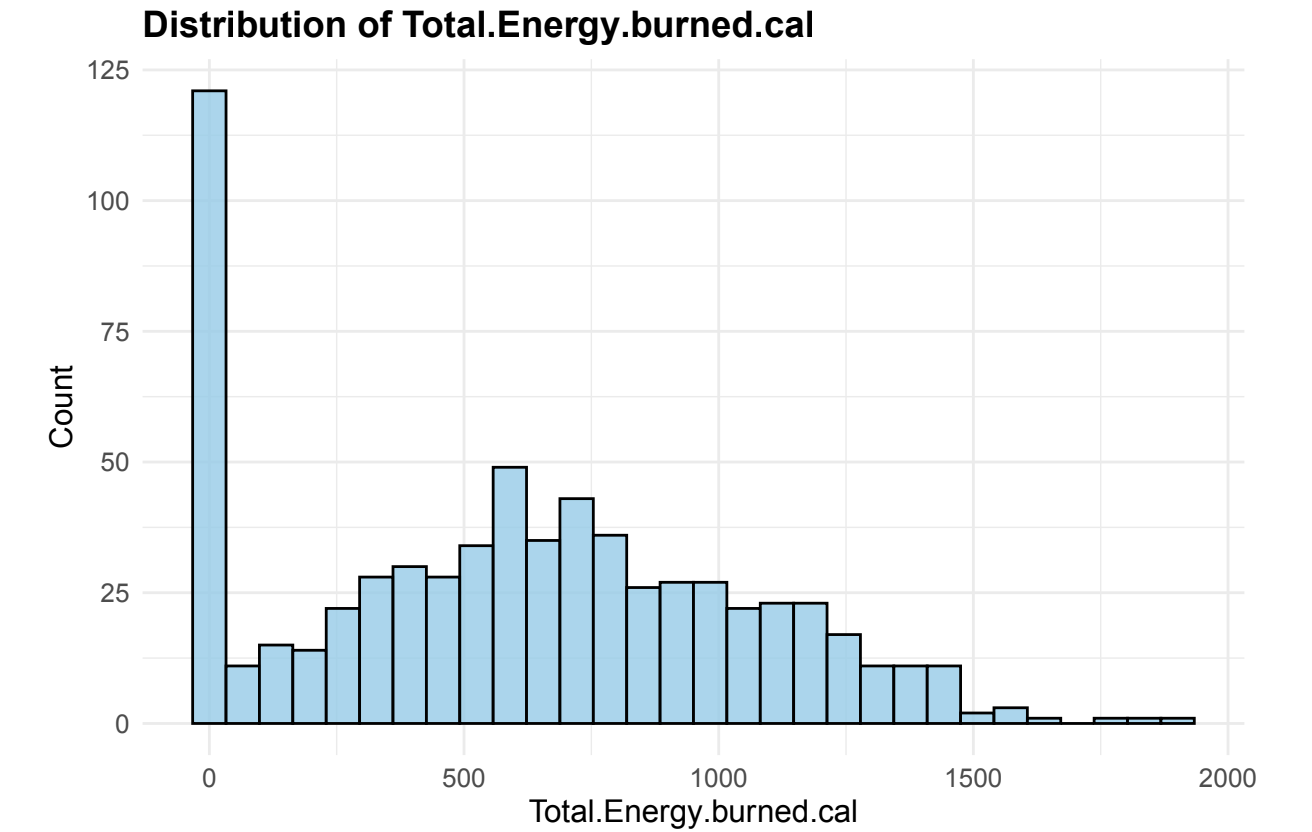
\includegraphics[width=0.6\textwidth]{images/Total_Energy_burned_cal.png}
  \caption{Distribution of Total.Energy.burned.cal}
  \label{fig:total_energy_burned}
\end{figure}

\begin{figure}[h!]
  \centering
  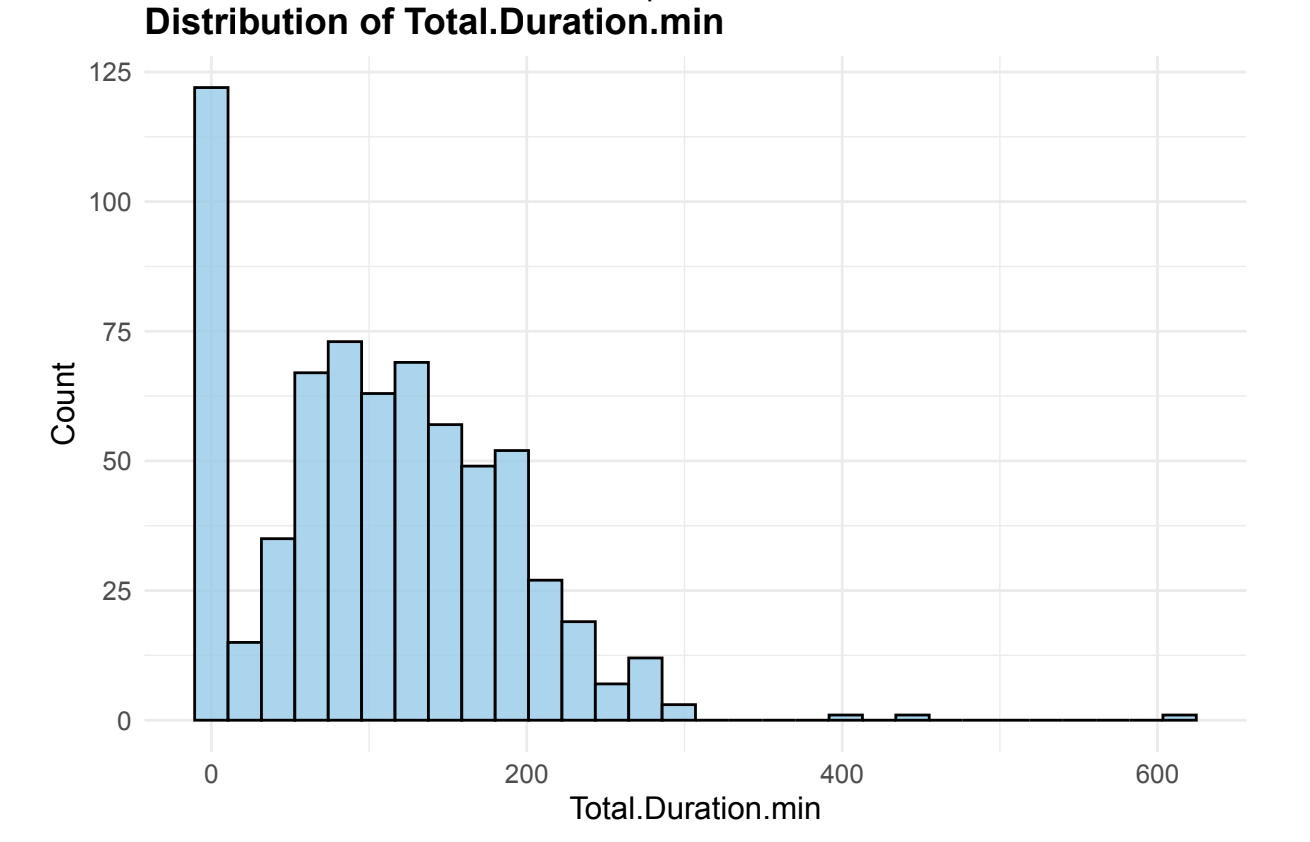
\includegraphics[width=0.6\textwidth]{images/Total_Duration_min.png}
  \caption{Distribution of Total.Duration.min}
  \label{fig:total_duration}
\end{figure}

\begin{figure}[h!]
  \centering
  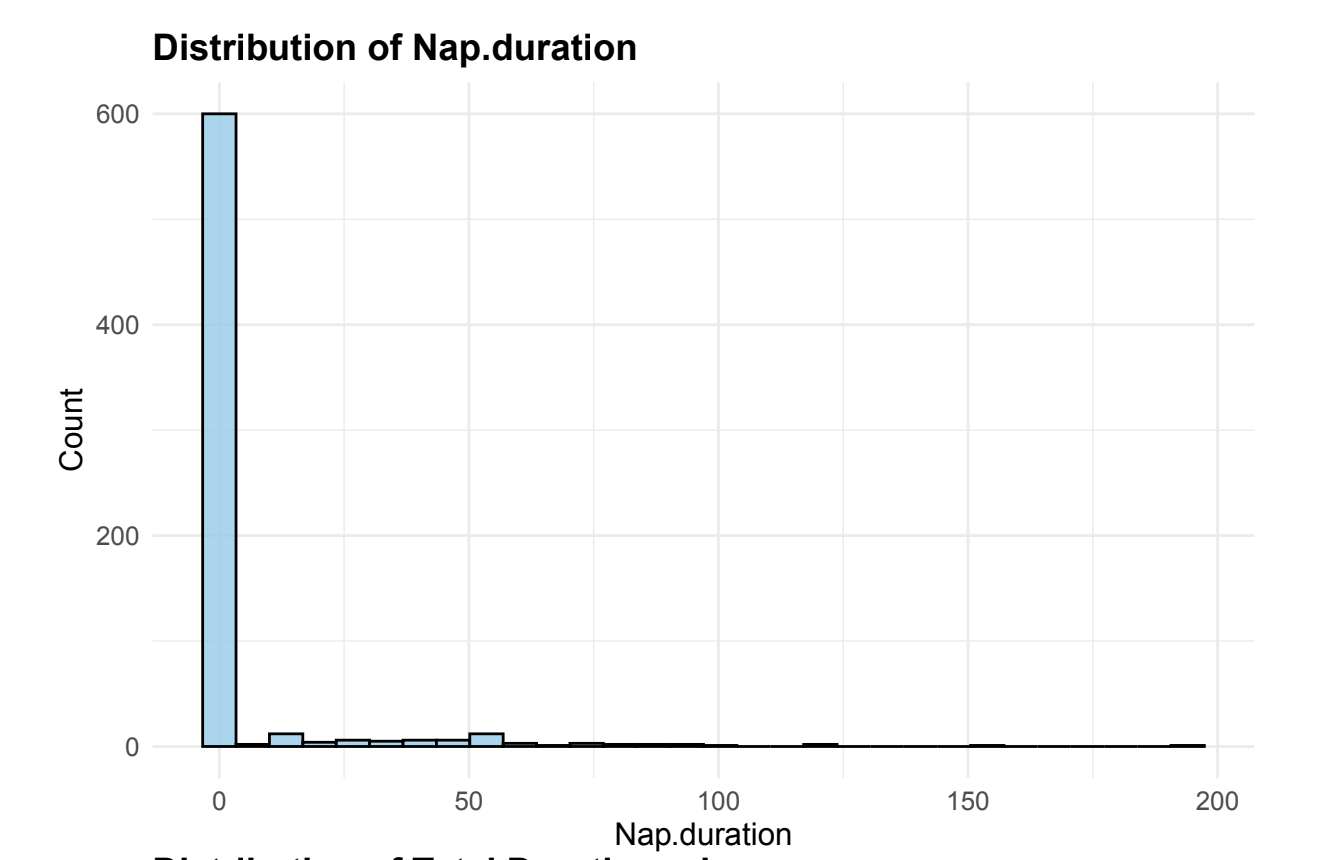
\includegraphics[width=0.6\textwidth]{images/Nap_duration.png}
  \caption{Distribution of Nap.duration}
  \label{fig:nap_duration}
\end{figure}

\begin{figure}[h!]
  \centering
  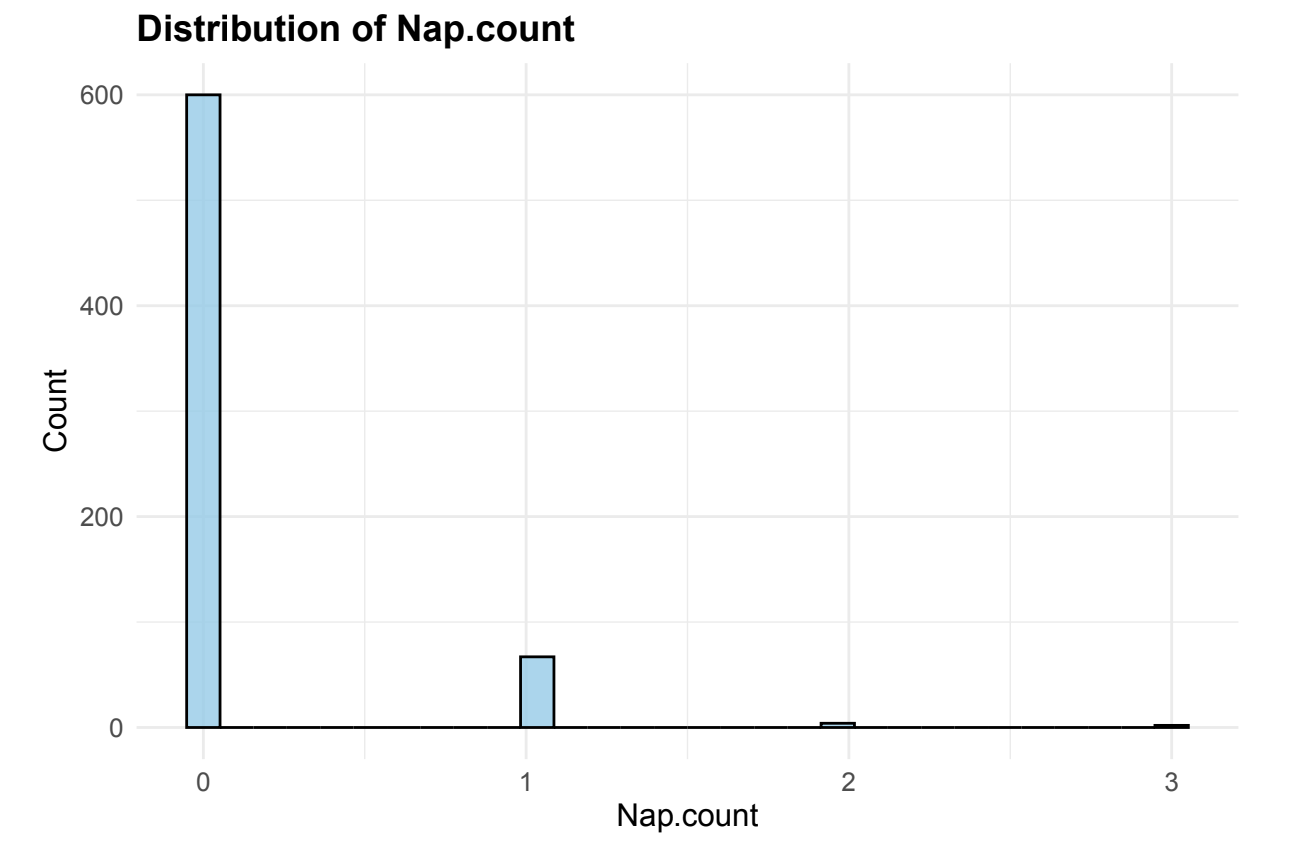
\includegraphics[width=0.6\textwidth]{images/Nap_count.png}
  \caption{Distribution of Nap.count}
  \label{fig:nap_count}
\end{figure}

\begin{figure}[h!]
  \centering
  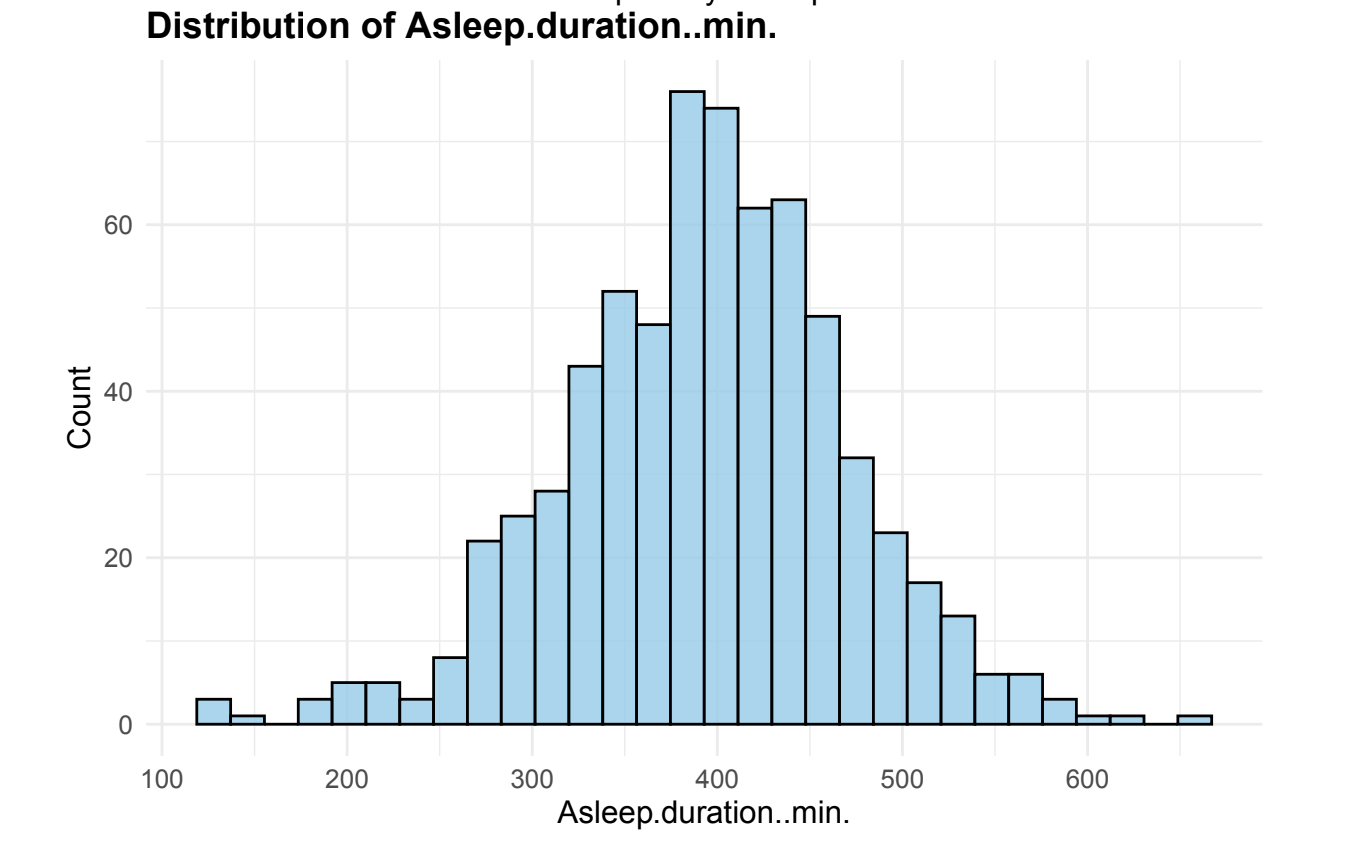
\includegraphics[width=0.6\textwidth]{images/Asleep_duration_min.png}
  \caption{Distribution of Asleep.duration..min.}
  \label{fig:asleep_duration}
\end{figure}

\begin{figure}[h!]
  \centering
  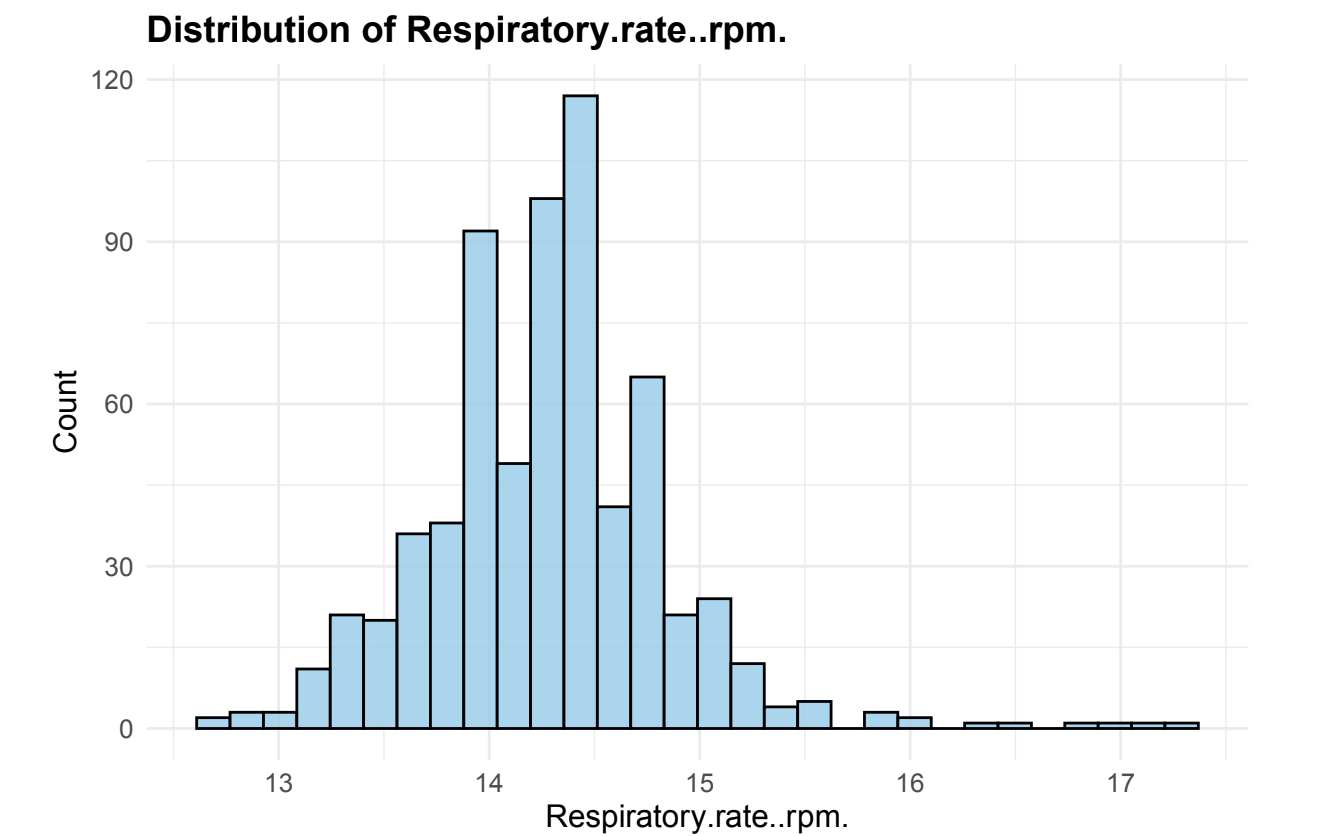
\includegraphics[width=0.6\textwidth]{images/Respiratory_rate_rpm.png}
  \caption{Distribution of Respiratory.rate..rpm.}
  \label{fig:respiratory_rate}
\end{figure}

\begin{figure}[h!]
  \centering
  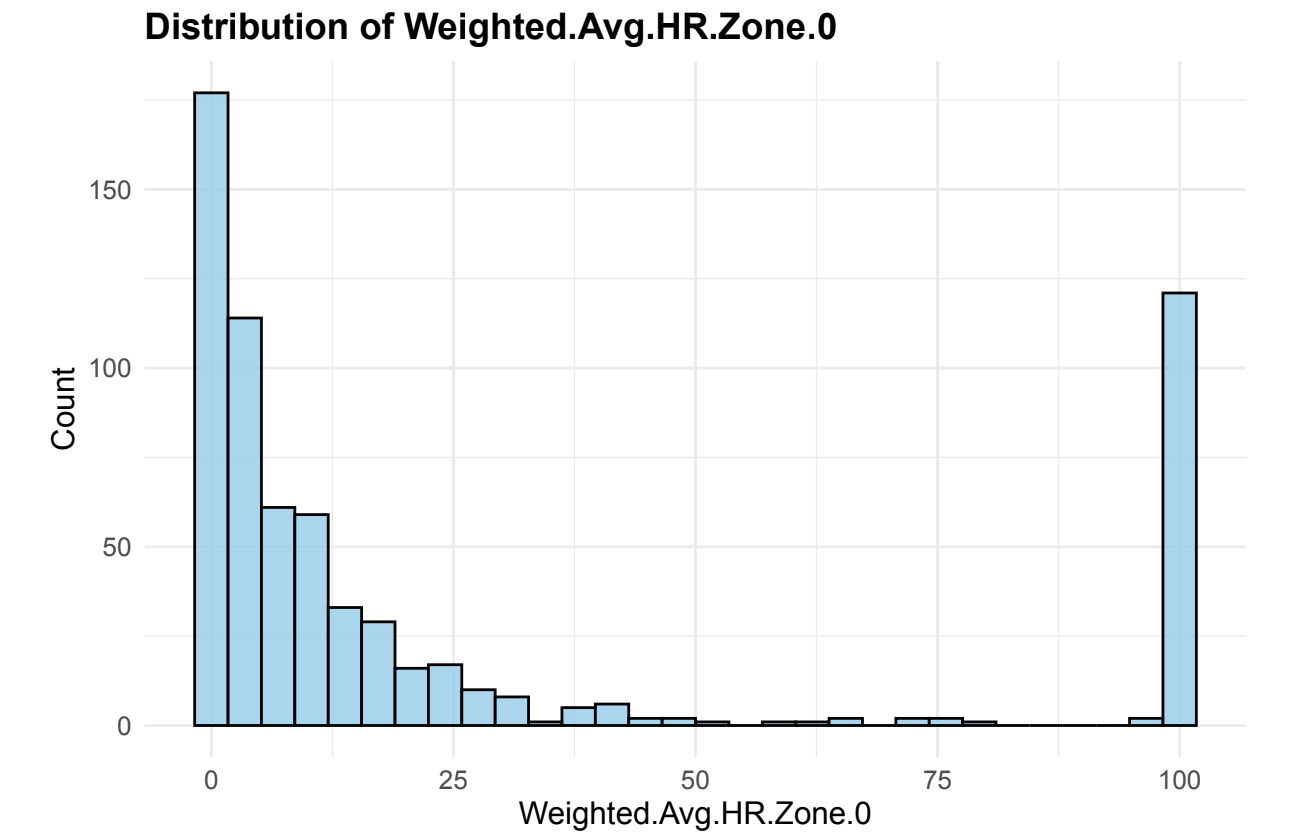
\includegraphics[width=0.6\textwidth]{images/Weighted_Avg_HR_Zone_0.png}
  \caption{Distribution of Weighted.Avg.HR.Zone.0}
  \label{fig:weighted_avg_hr_zone_0}
\end{figure}

\begin{figure}[h!]
  \centering
  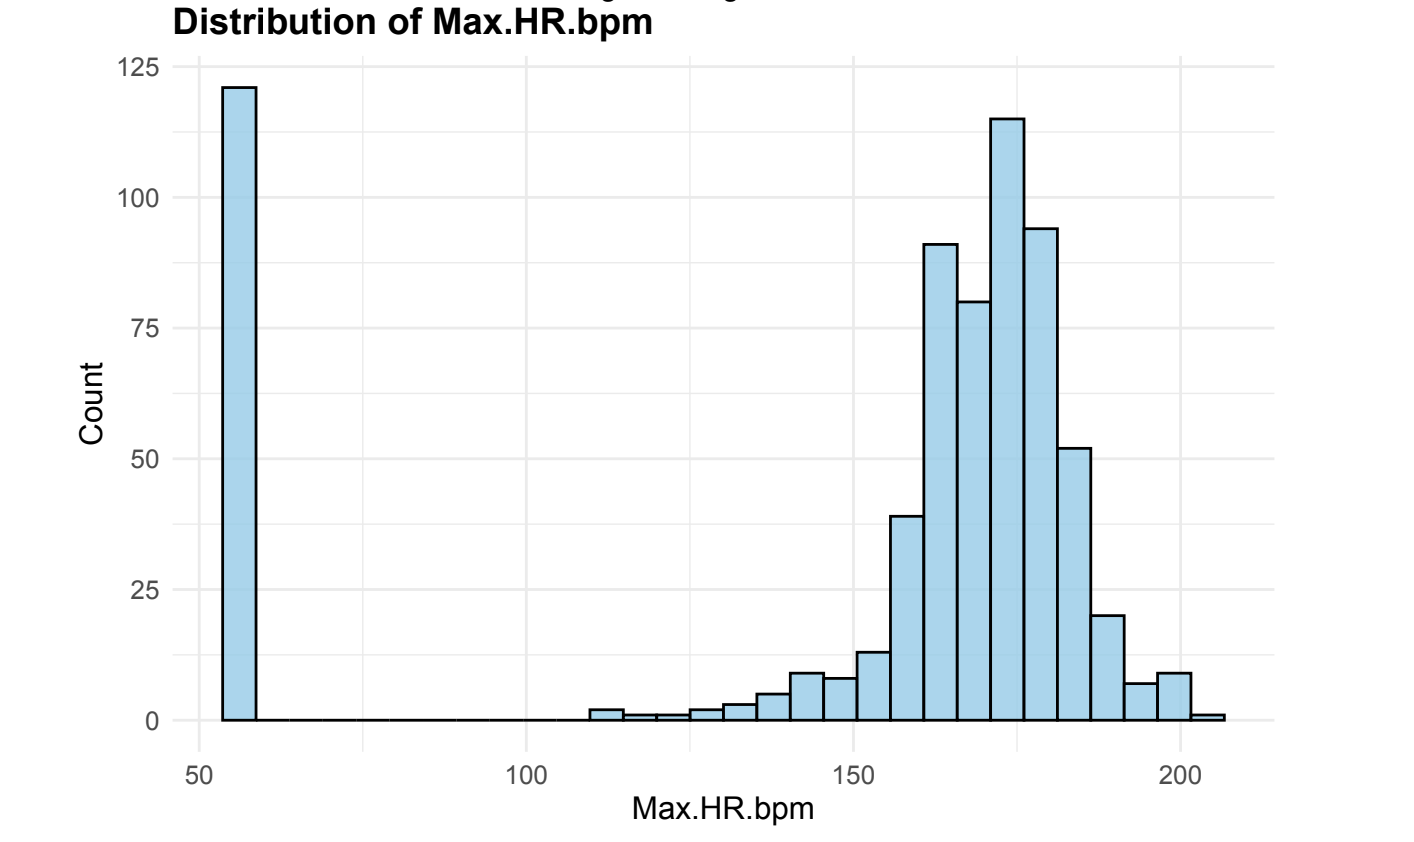
\includegraphics[width=0.6\textwidth]{images/Max_HR_bpm.png}
  \caption{Distribution of Max.HR.bpm}
  \label{fig:max_hr_bpm}
\end{figure}

\begin{figure}[h!]
  \centering
  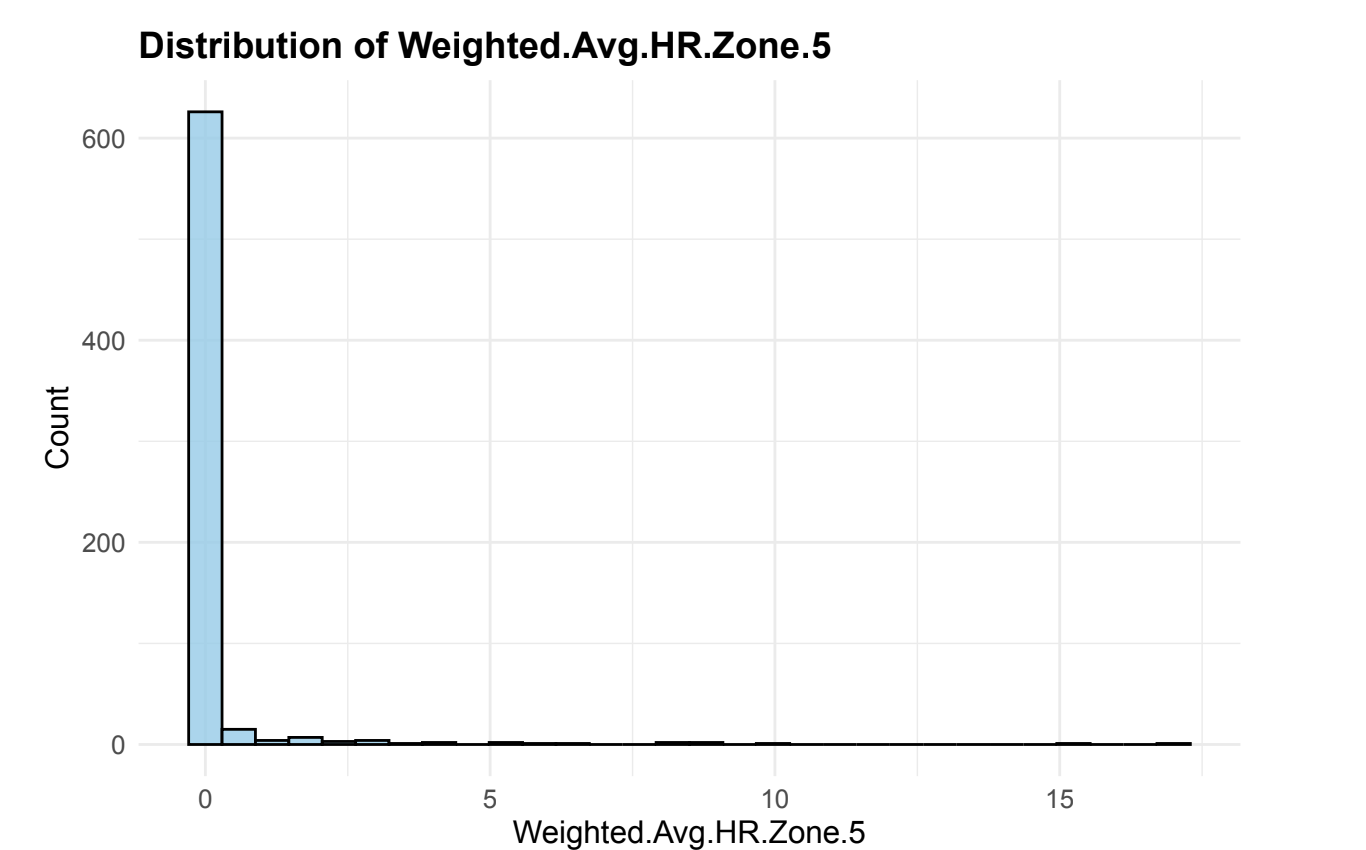
\includegraphics[width=0.6\textwidth]{images/Weighted_Avg_HR_Zone_5.png}
  \caption{Distribution of Weighted.Avg.HR.Zone.5}
  \label{fig:weighted_avg_hr_zone_5}
\end{figure}

\begin{figure}[h!]
  \centering
  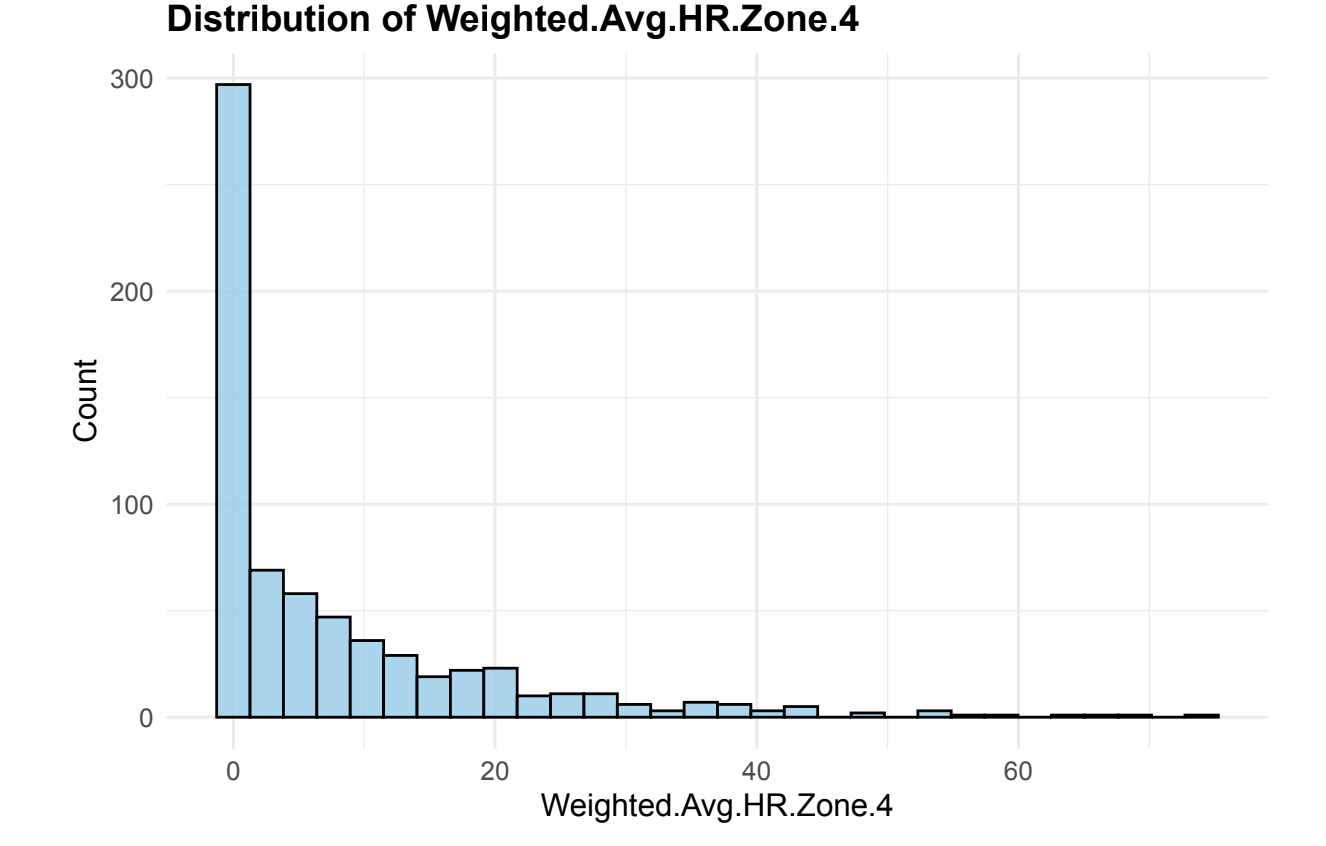
\includegraphics[width=0.6\textwidth]{images/Weighted_Avg_HR_Zone_4.png}
  \caption{Distribution of Weighted.Avg.HR.Zone.4}
  \label{fig:weighted_avg_hr_zone_4}
\end{figure}

\begin{figure}[h!]
  \centering
  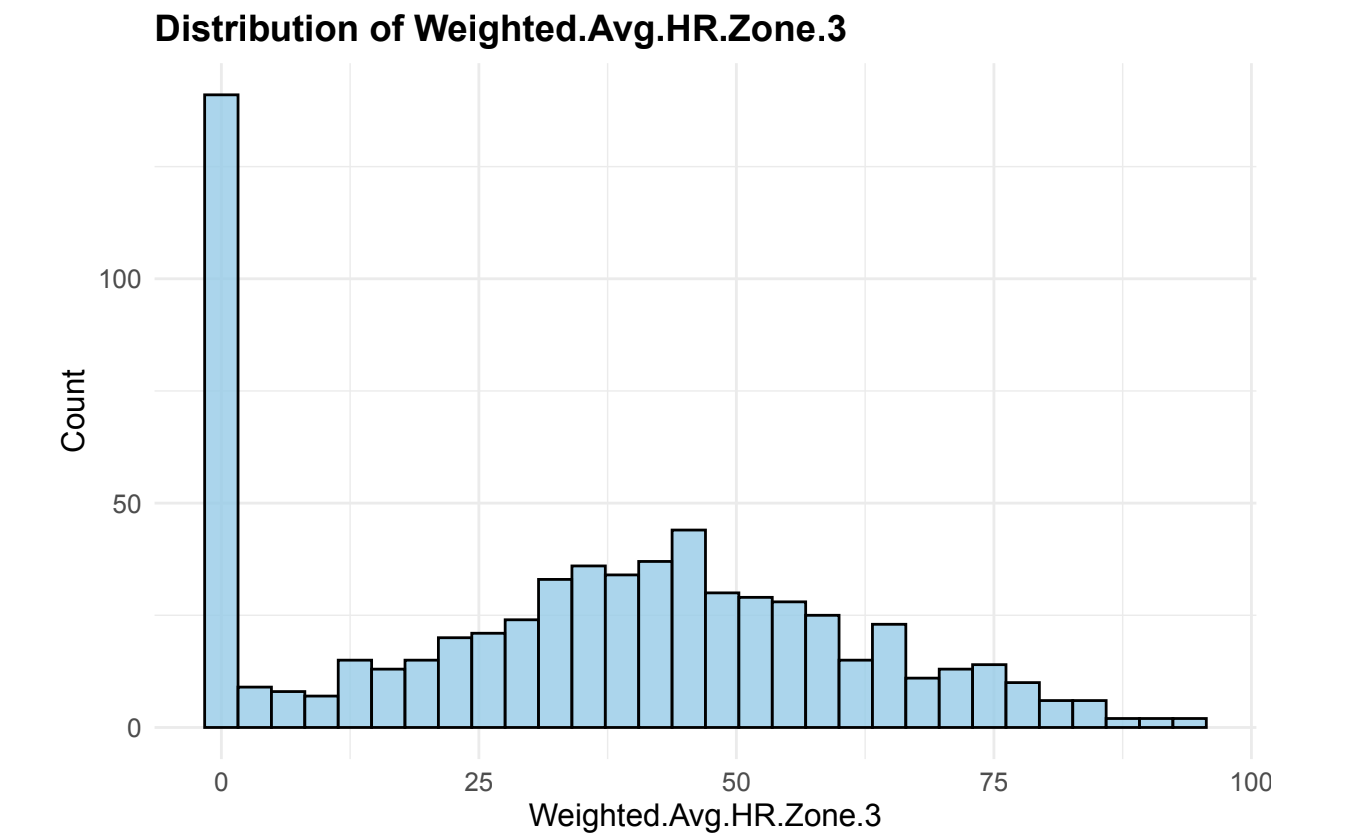
\includegraphics[width=0.6\textwidth]{images/Weighted_Avg_HR_Zone_3.png}
  \caption{Distribution of Weighted.Avg.HR.Zone.3}
  \label{fig:weighted_avg_hr_zone_3}
\end{figure}

\begin{figure}[h!]
  \centering
  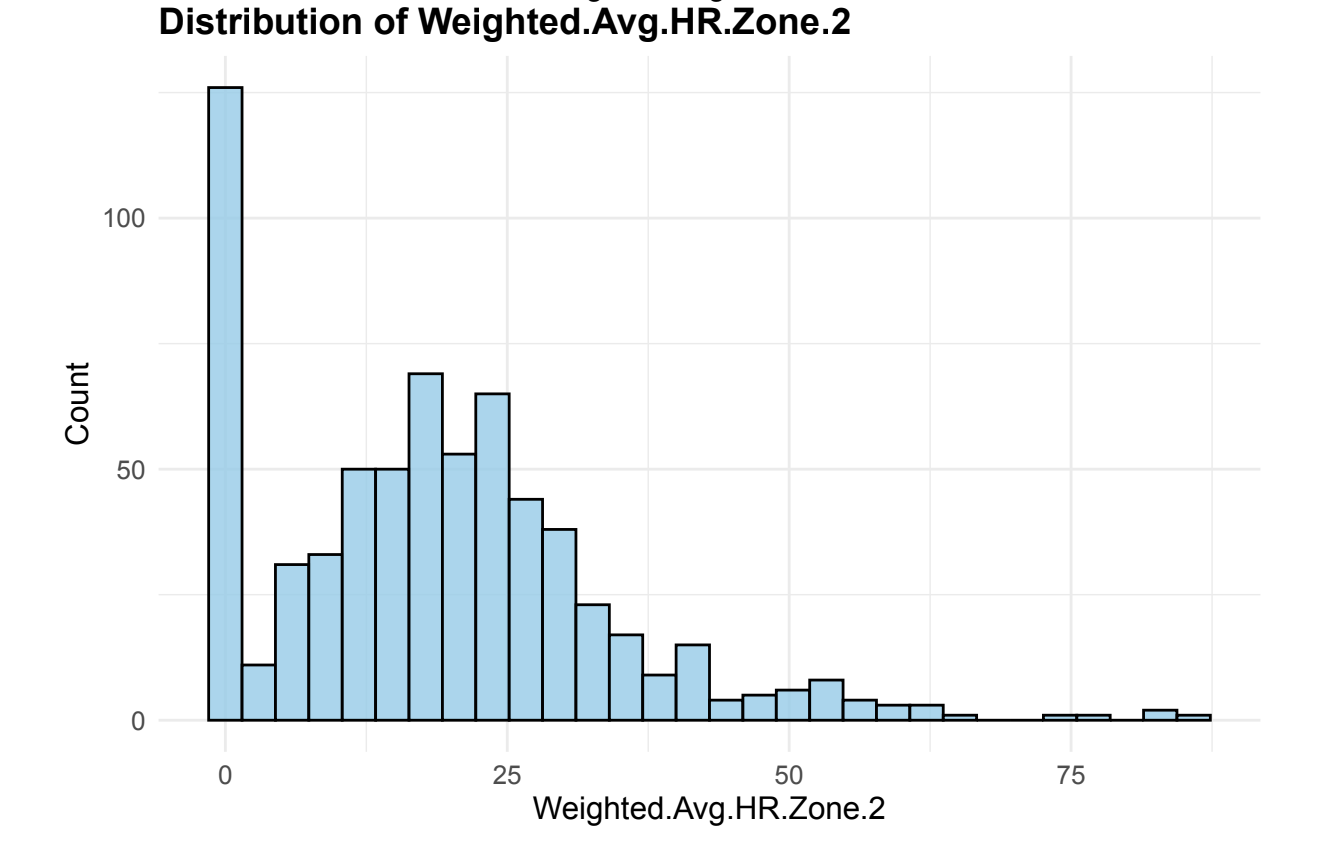
\includegraphics[width=0.6\textwidth]{images/Weighted_Avg_HR_Zone_2.png}
  \caption{Distribution of Weighted.Avg.HR.Zone.2}
  \label{fig:weighted_avg_hr_zone_2}
\end{figure}

\begin{figure}[h!]
  \centering
  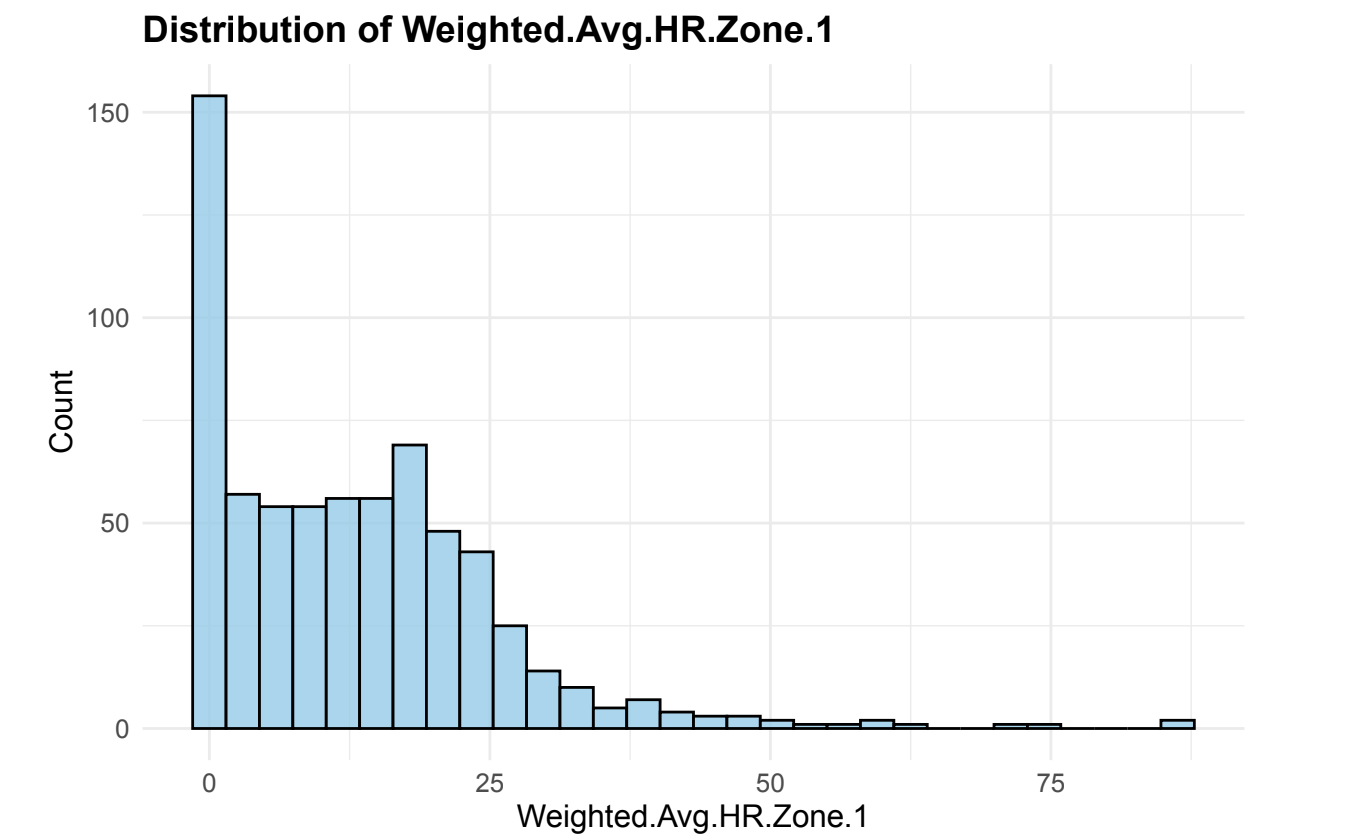
\includegraphics[width=0.6\textwidth]{images/Weighted_Avg_HR_Zone_1.png}
  \caption{Distribution of Weighted.Avg.HR.Zone.1}
  \label{fig:weighted_avg_hr_zone_1}
\end{figure}

\begin{figure}[h!]
  \centering
  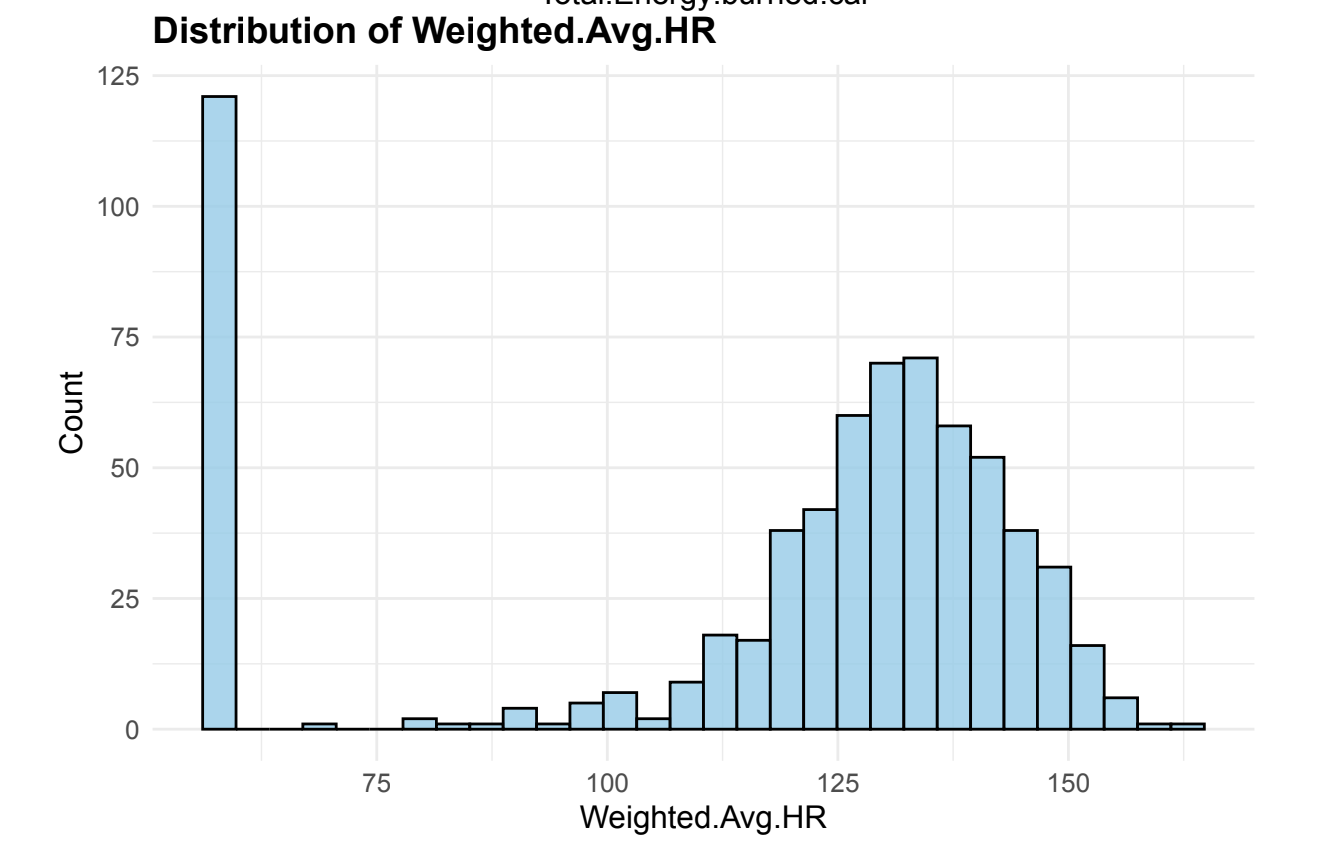
\includegraphics[width=0.6\textwidth]{images/Weighted_Avg_HR.png}
  \caption{Distribution of Weighted.Avg.HR}
  \label{fig:weighted_avg_hr}
\end{figure}

\newpage

% General Model Plot: Residuals vs Fitted
\begin{figure}[h!]
  \centering
  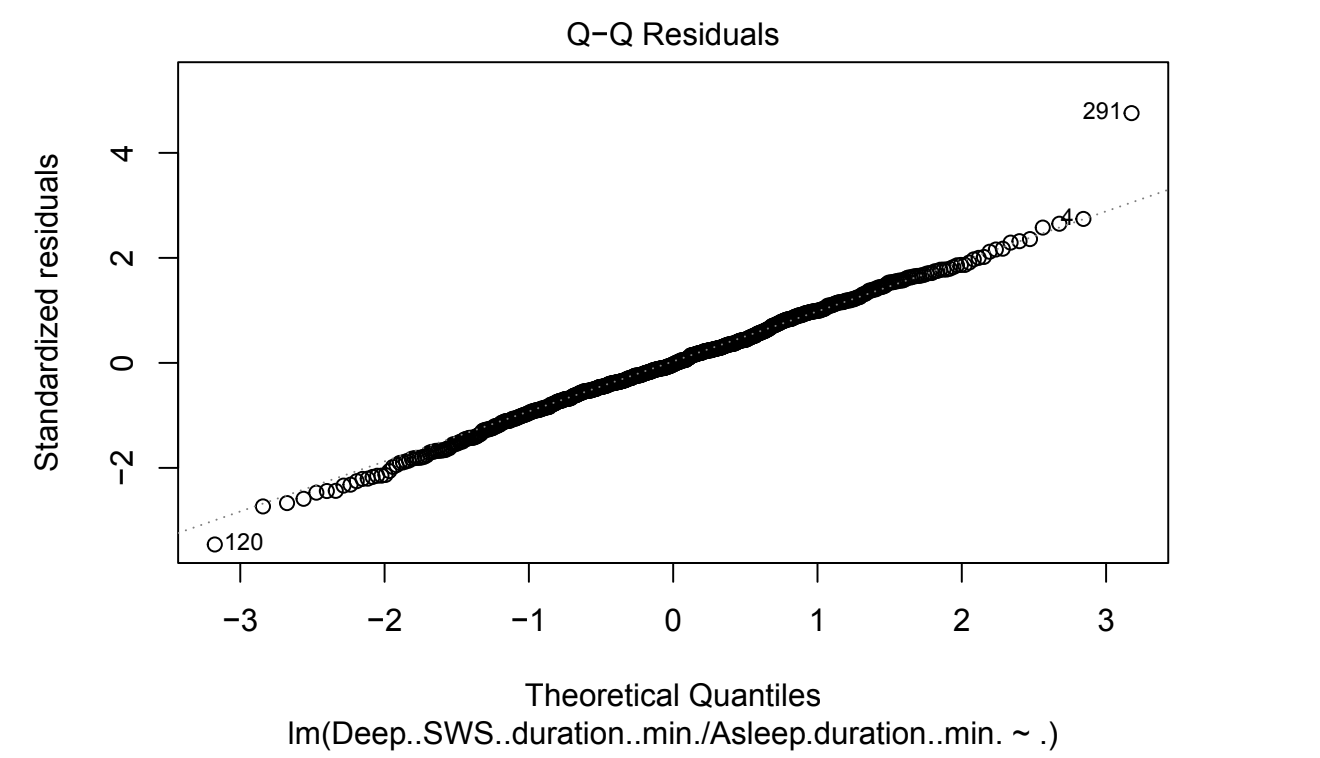
\includegraphics[width=0.7\textwidth]{images/model_plot1.png}
  \caption{General Model: Residuals vs Fitted}
  \label{fig:general_residuals_vs_fitted}
\end{figure}

% General Model Plot: Q-Q Residuals
\begin{figure}[h!]
  \centering
  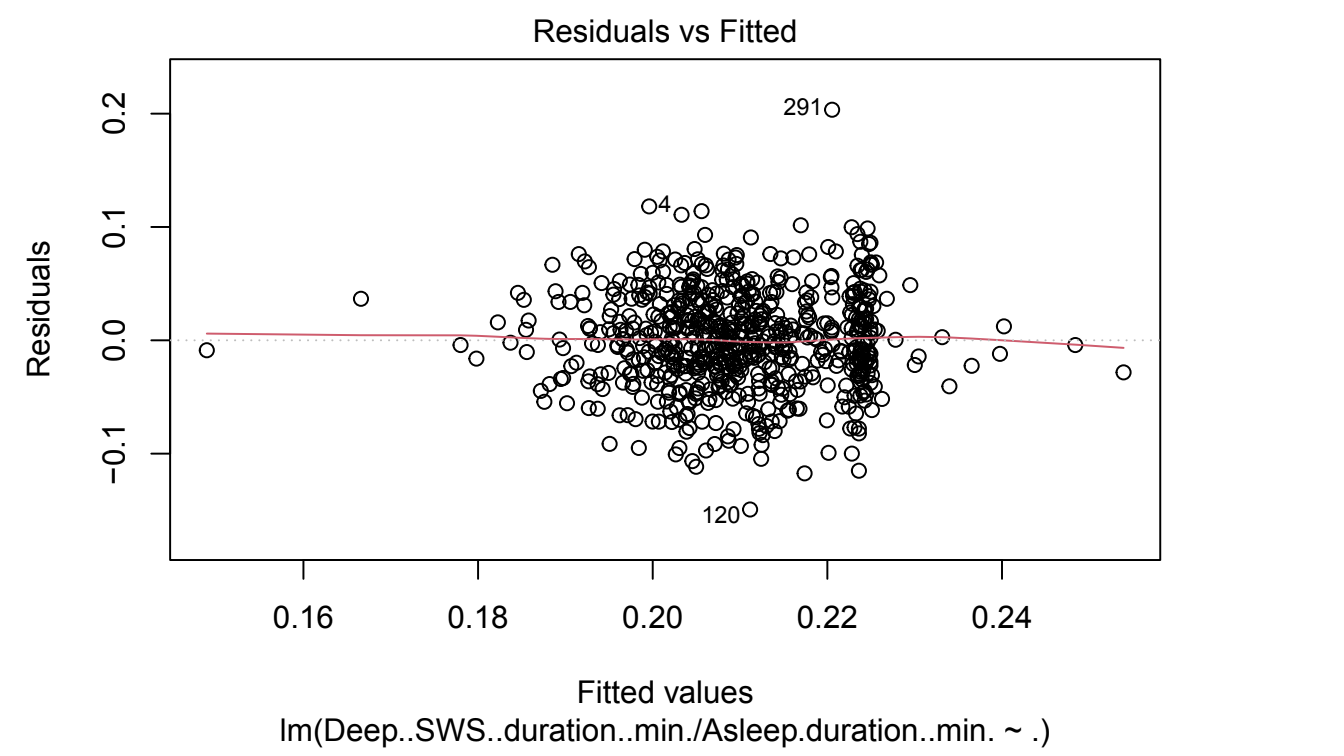
\includegraphics[width=0.7\textwidth]{images/model_plot2.png}
  \caption{General Model: Q-Q Residuals}
  \label{fig:general_qq_residuals}
\end{figure}

% Interactions Model Plot: Residuals vs Fitted
\begin{figure}[h!]
  \centering
  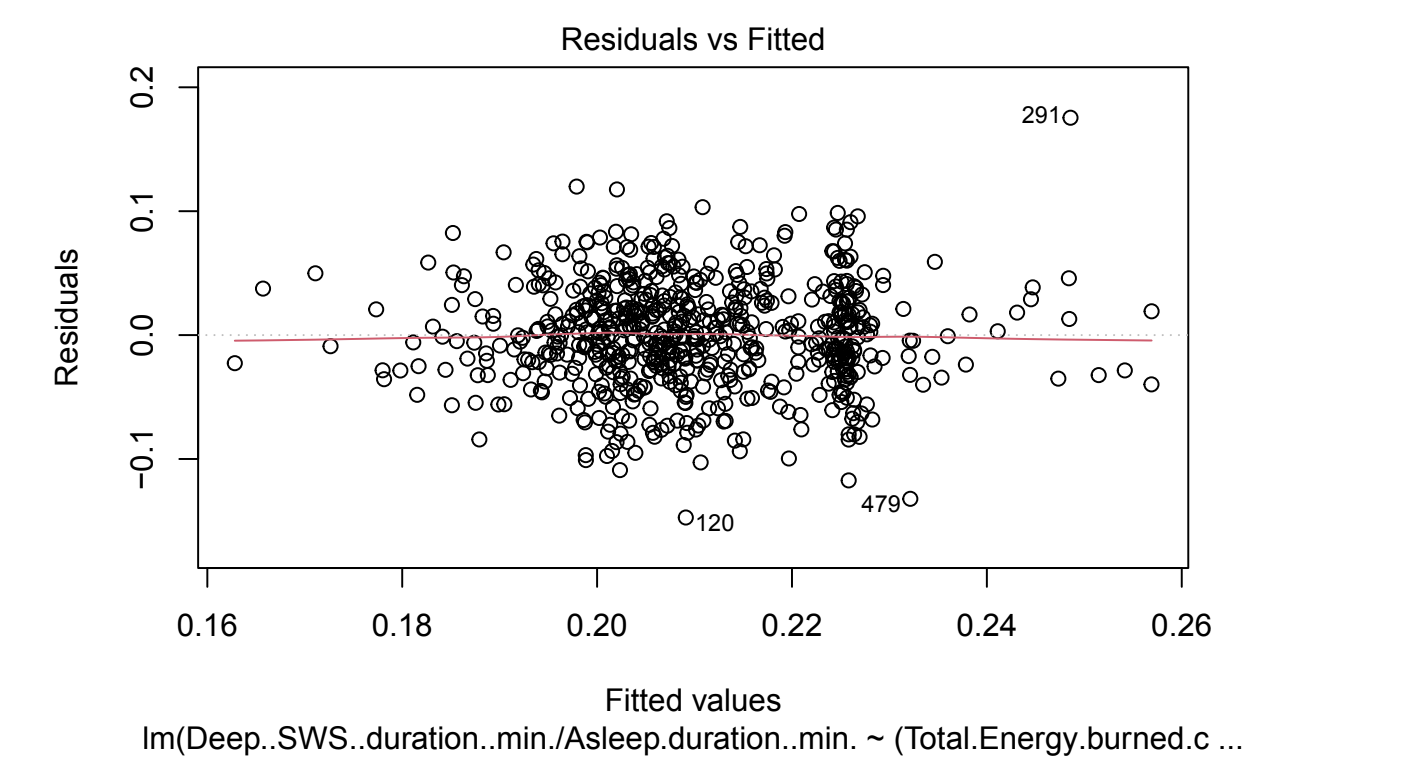
\includegraphics[width=0.7\textwidth]{images/model_rr_plot1.png}
  \caption{Interactions Model: Residuals vs Fitted}
  \label{fig:interactions_residuals_vs_fitted}
\end{figure}

% Interactions Model Plot: Q-Q Residuals
\begin{figure}[h!]
  \centering
  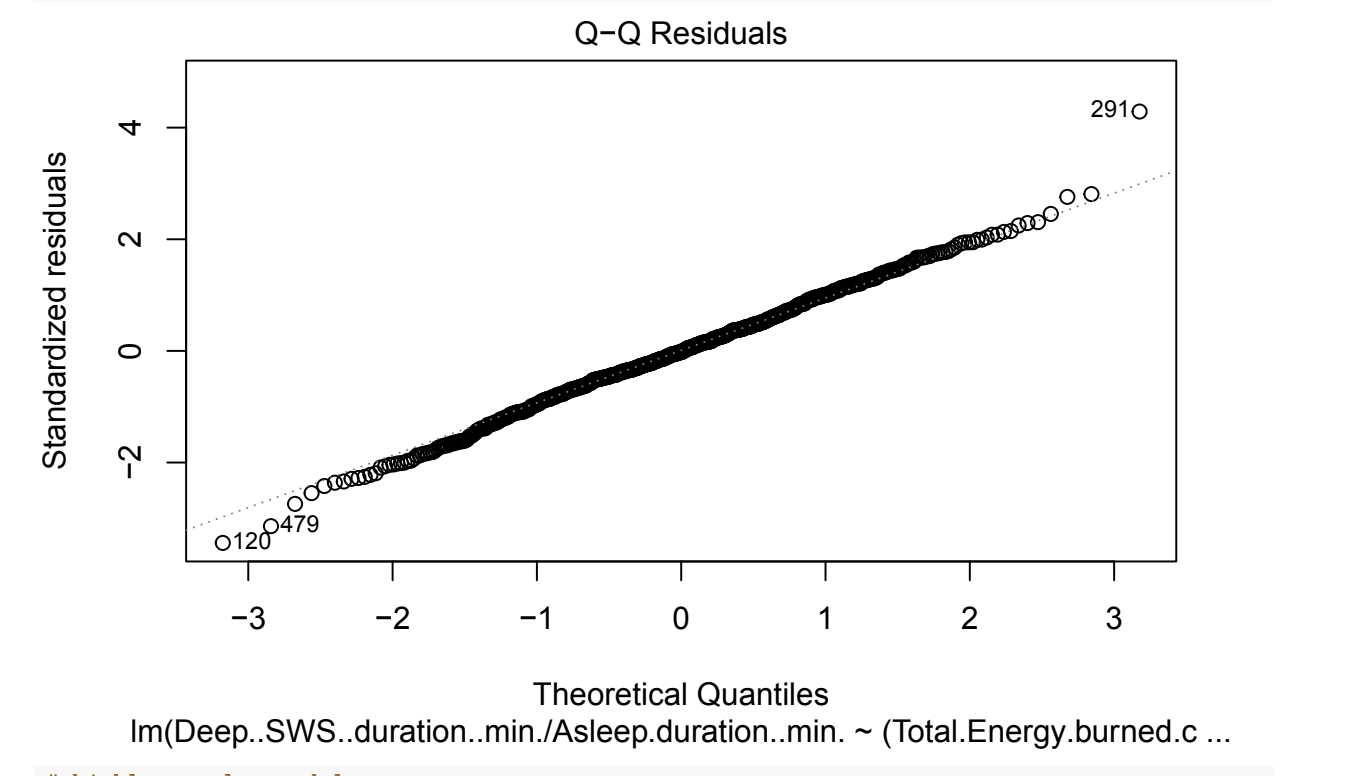
\includegraphics[width=0.7\textwidth]{images/model_rr_plot2.png}
  \caption{Interactions Model: Q-Q Residuals}
  \label{fig:I=interactions_qq_residuals}
\end{figure}

% Full Model Plot: Residuals vs Fitted
\begin{figure}[h!]
  \centering
  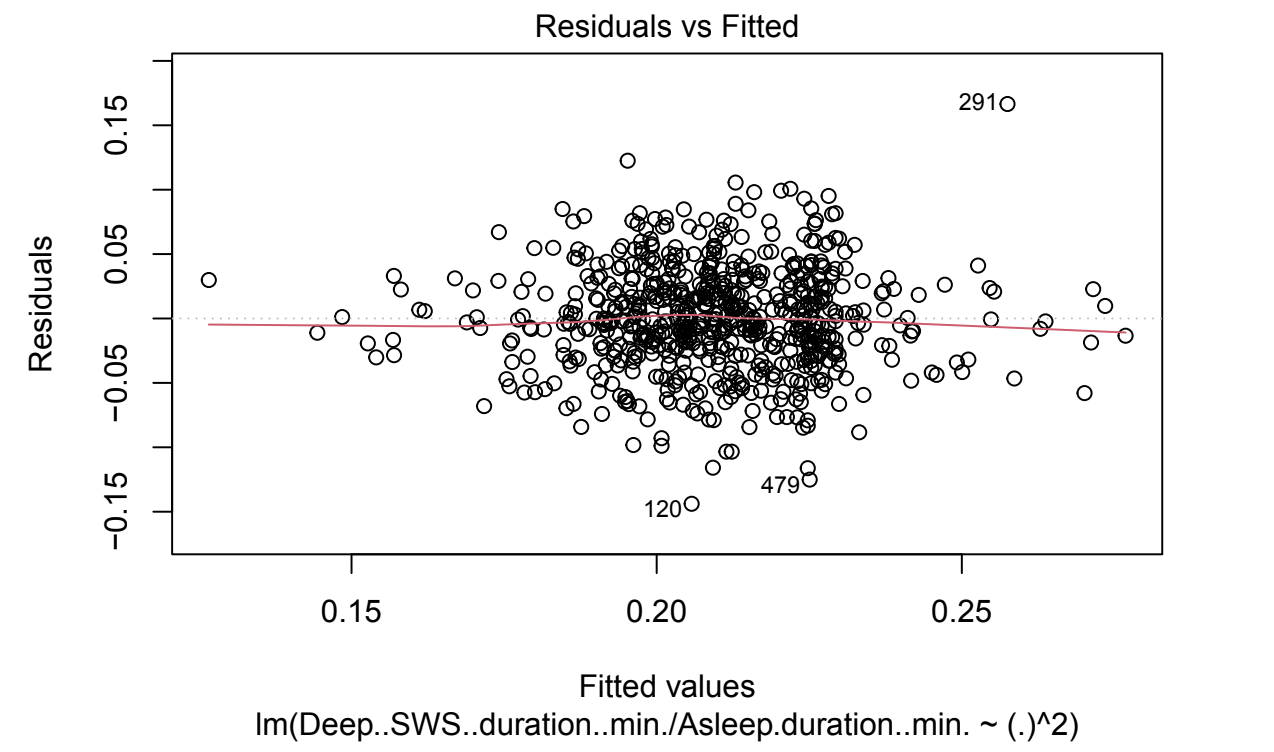
\includegraphics[width=0.7\textwidth]{images/model_full_plot1.png}
  \caption{Full Model: Residuals vs Fitted}
  \label{fig:full_residuals_vs_fitted}
\end{figure}
% Full Model Plot: Q-Q Residuals
\begin{figure}[h!]
  \centering
  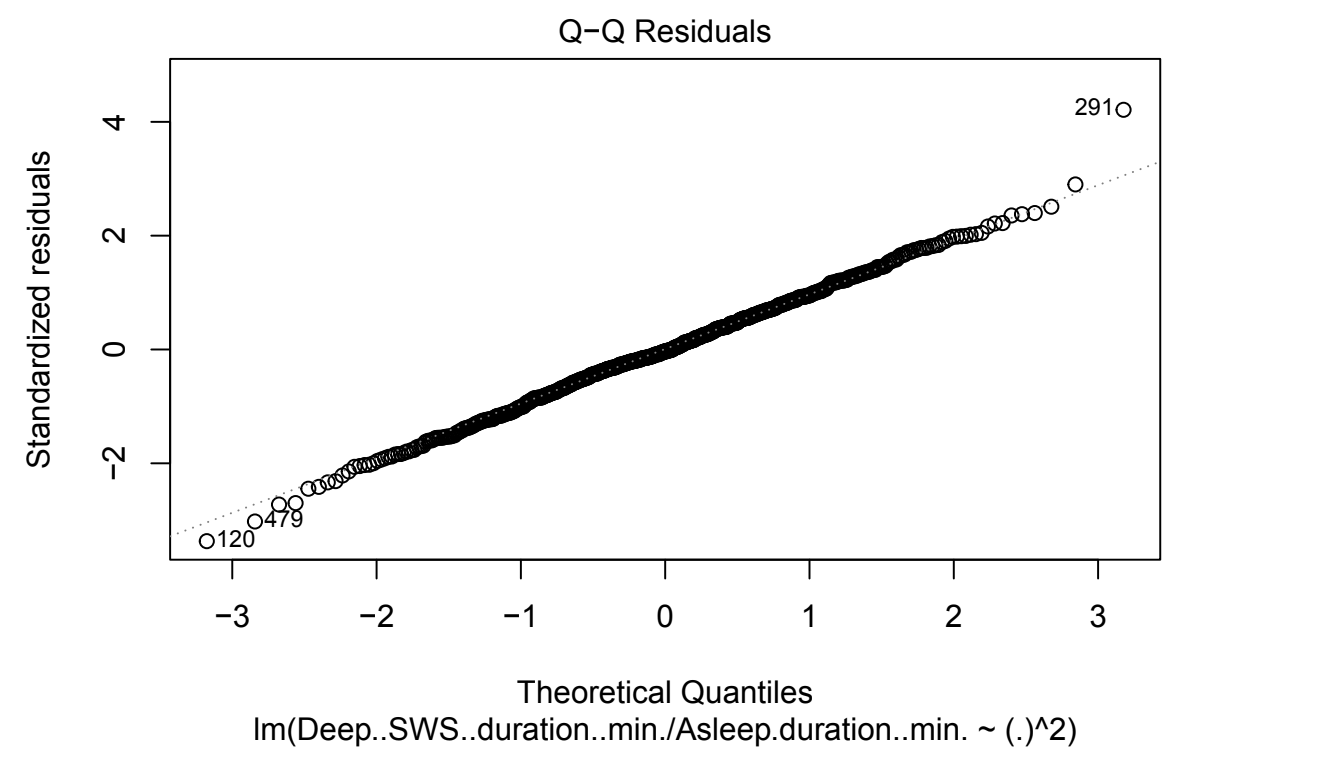
\includegraphics[width=0.7\textwidth]{images/model_full_plot2.png}
  \caption{Full Model: Q-Q Residuals}
  \label{fig:full_qq_residuals}
\end{figure}

% Model Selection
% Backward Selection: Residuals vs Fitted
\begin{figure}[h!]
  \centering
  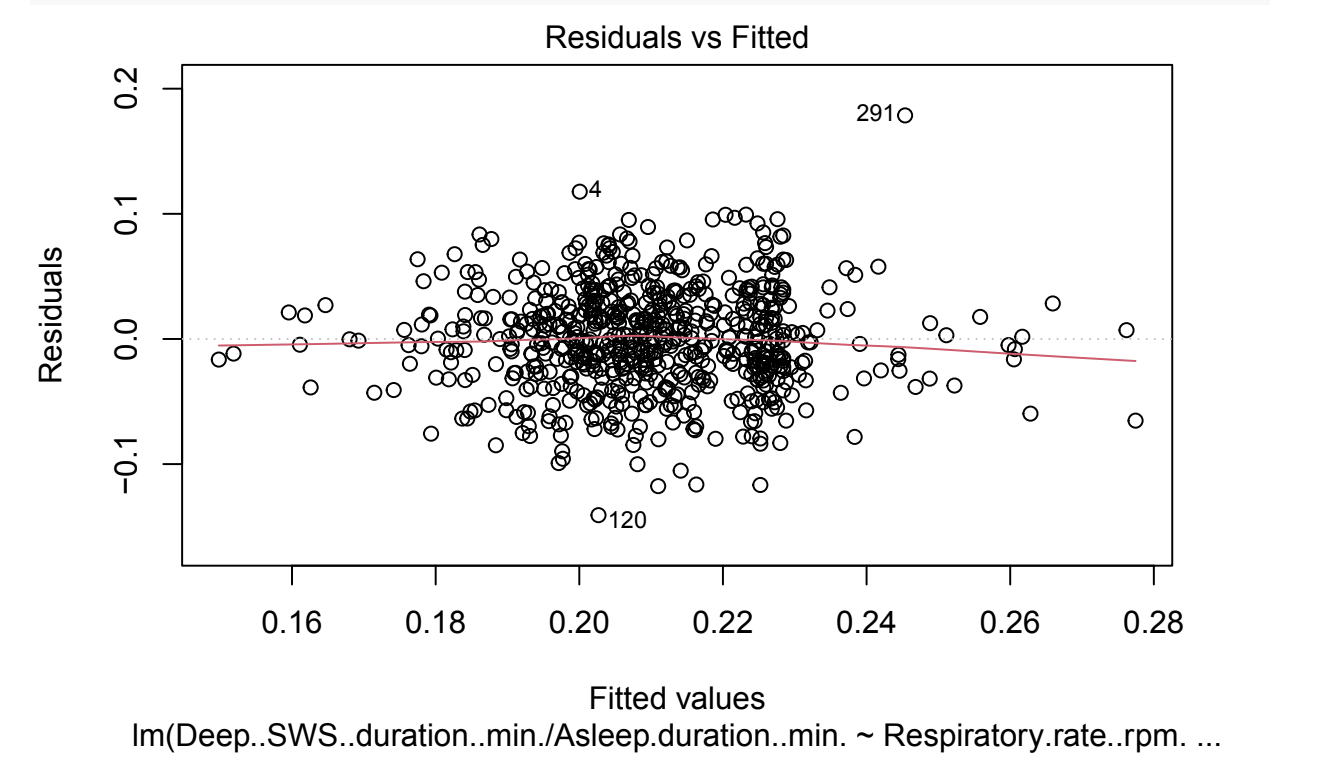
\includegraphics[width=0.6\textwidth]{images/selection_backward_plot1.png}
  \caption{Model Selection (Backward): Residuals vs Fitted}
  \label{fig:backward_residuals_vs_fitted}
\end{figure}

% Backward Selection: Q-Q Residuals
\begin{figure}[h!]
  \centering
  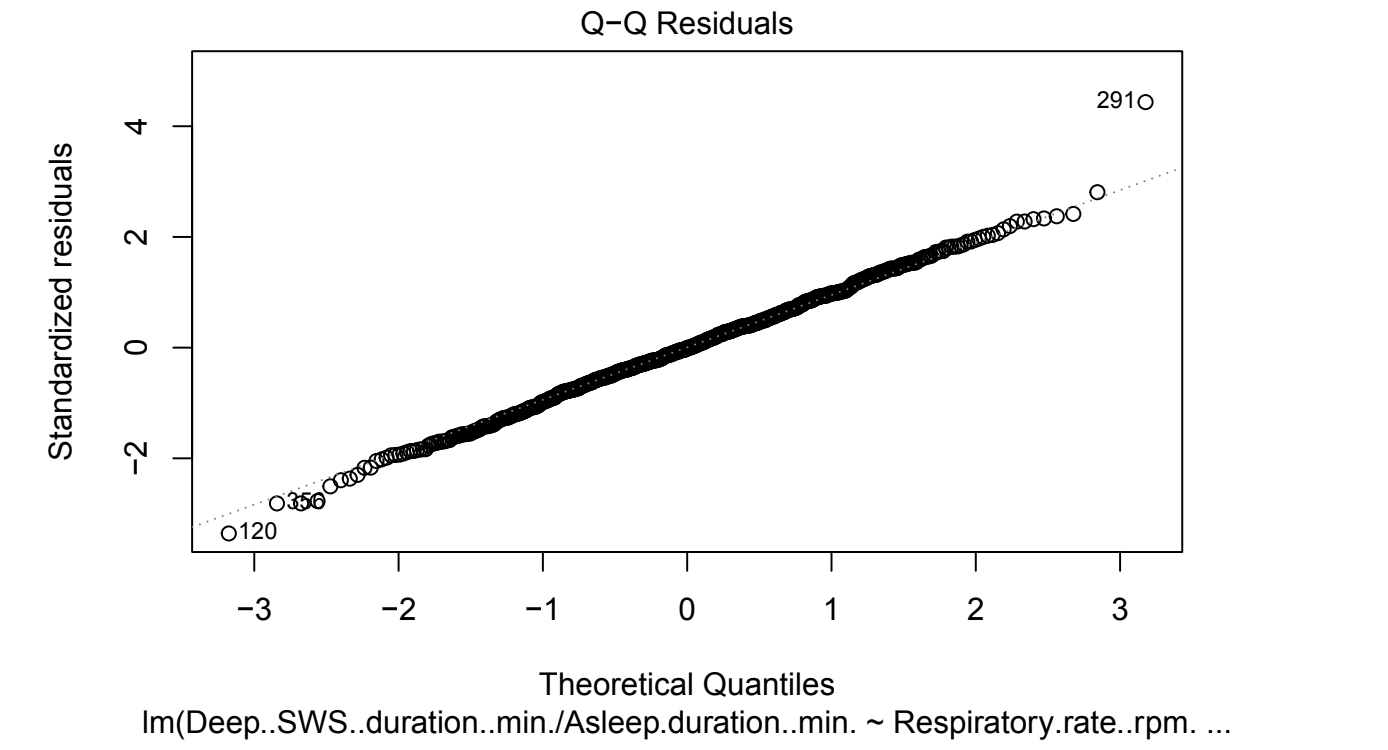
\includegraphics[width=0.6\textwidth]{images/selection_backward_plot2.png}
  \caption{Model Selection (Backward): Q-Q Residuals}
  \label{fig:backward_qq_residuals}
\end{figure}

% Forward Selection: Residuals vs Fitted
\begin{figure}[h!]
  \centering
  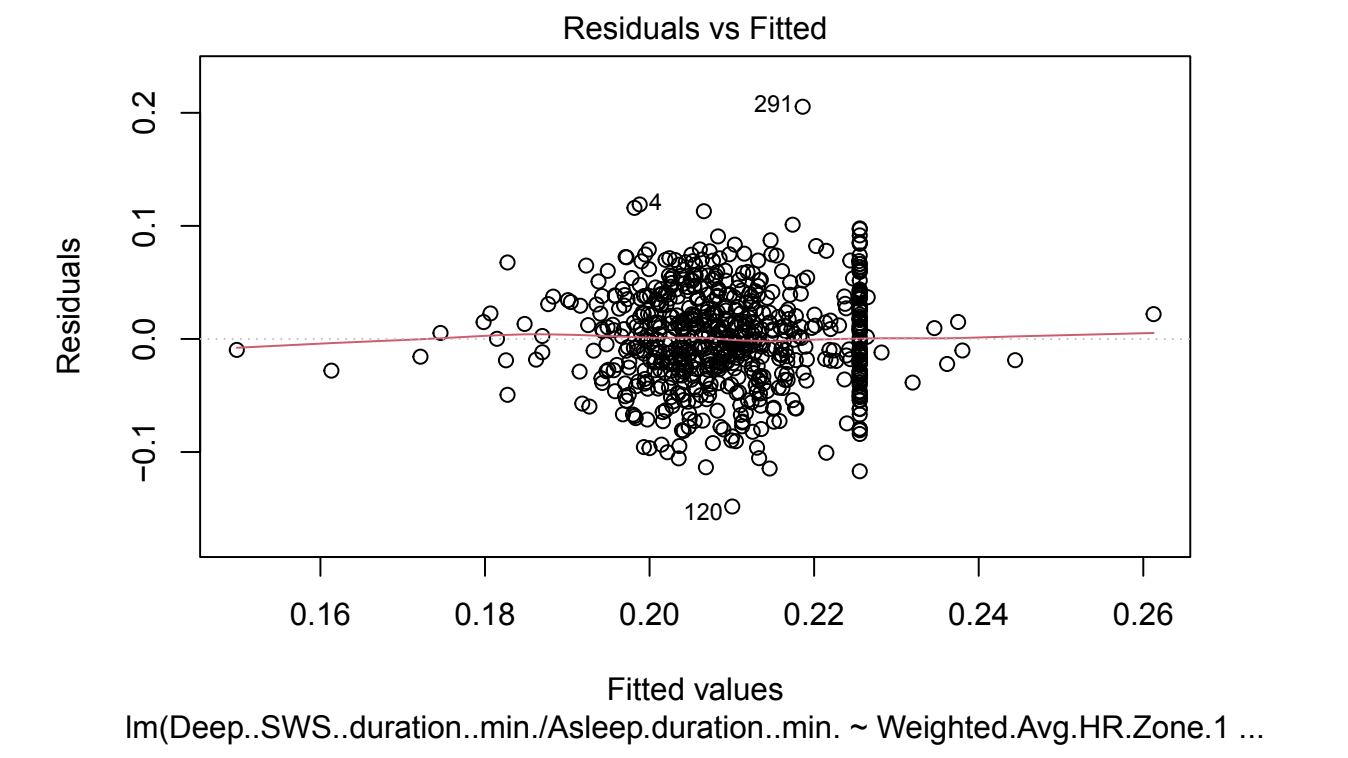
\includegraphics[width=0.6\textwidth]{images/selection_forward_plot1.png}
  \caption{Model Selection (Forward): Residuals vs Fitted}
  \label{fig:forward_residuals_vs_fitted}
\end{figure}

% Forward Selection: Q-Q Residuals
\begin{figure}[h!]
  \centering
  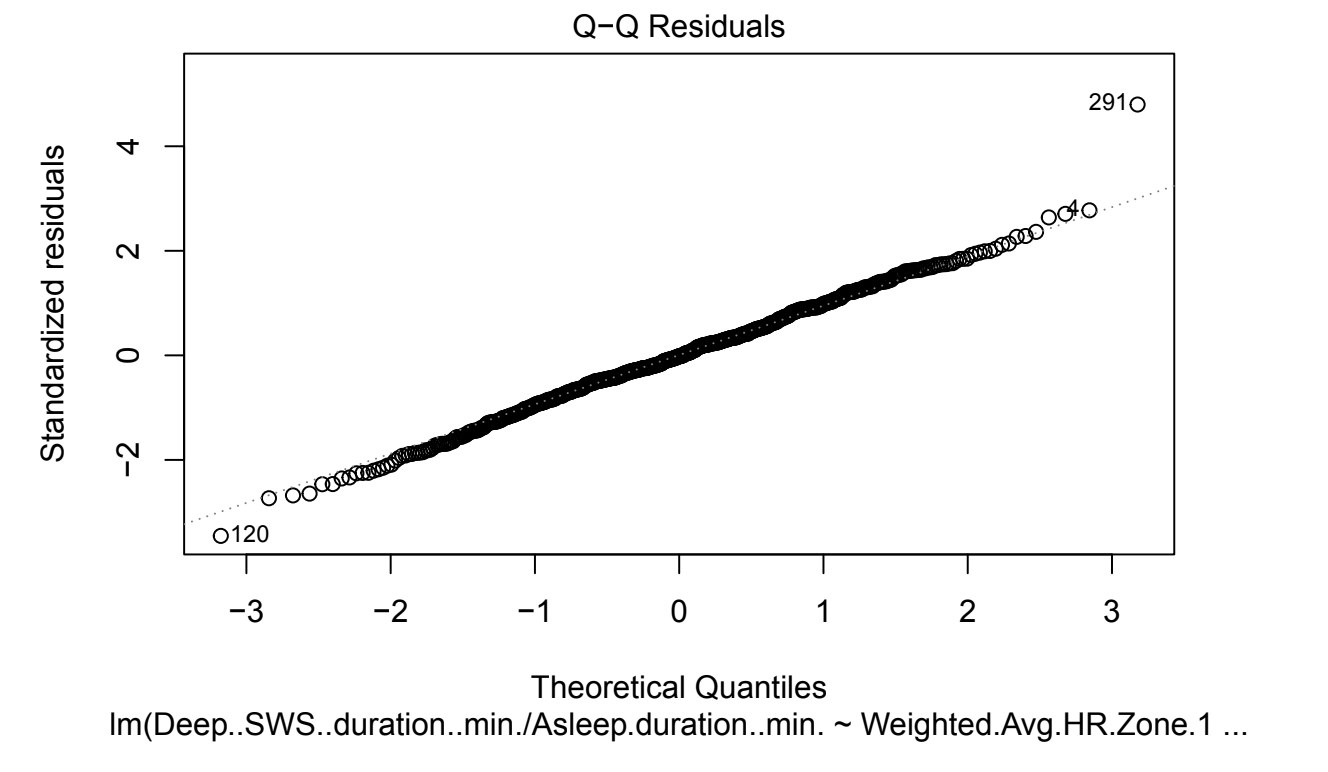
\includegraphics[width=0.6\textwidth]{images/selection_forward_plot2.png}
  \caption{Model Selection (Forward): Q-Q Residuals}
  \label{fig:forward_qq_residuals}
\end{figure}

\begin{figure}[h!]
  \centering
  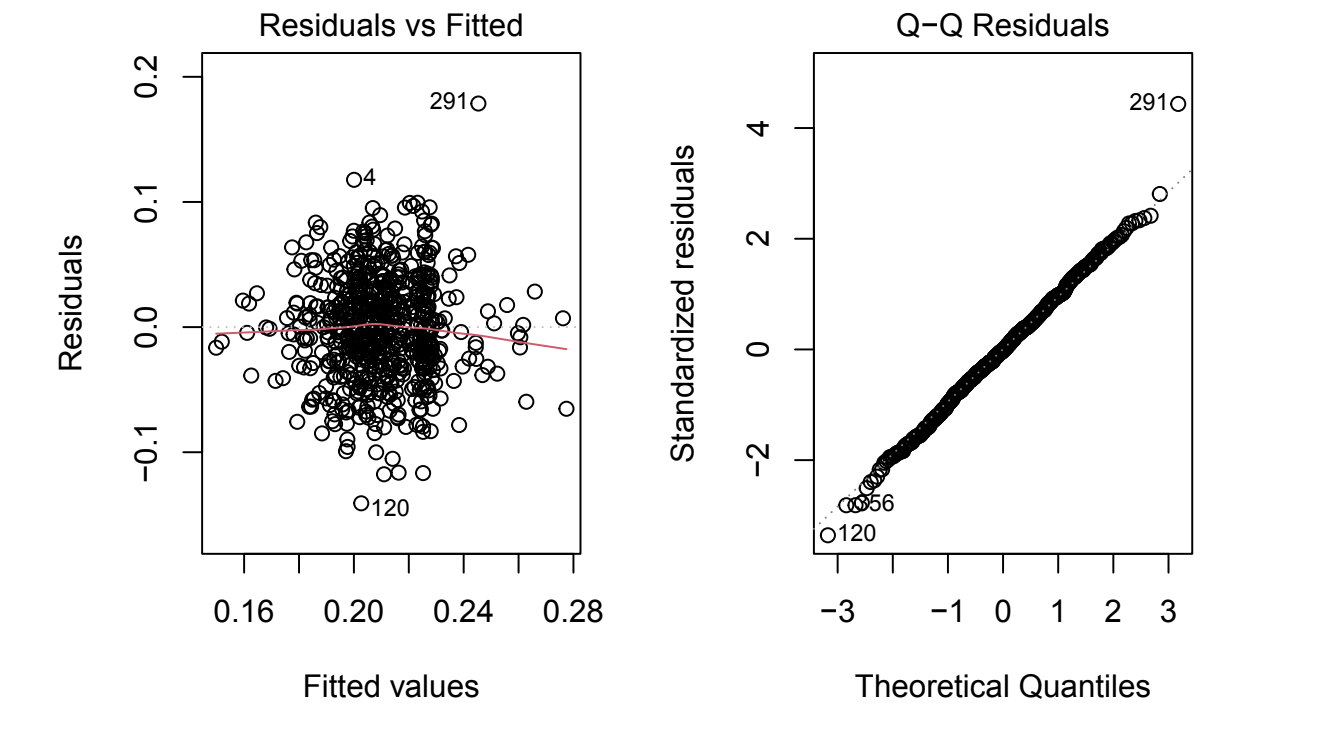
\includegraphics[width=0.6\textwidth]{images/pred_model_backward_plot1.png}
  \caption{Prediction: Residuals vs Total Duration and Histogram of Residuals}
  \label{fig:residuals_total_duration}
\end{figure}

\begin{figure}[h!]
  \centering
  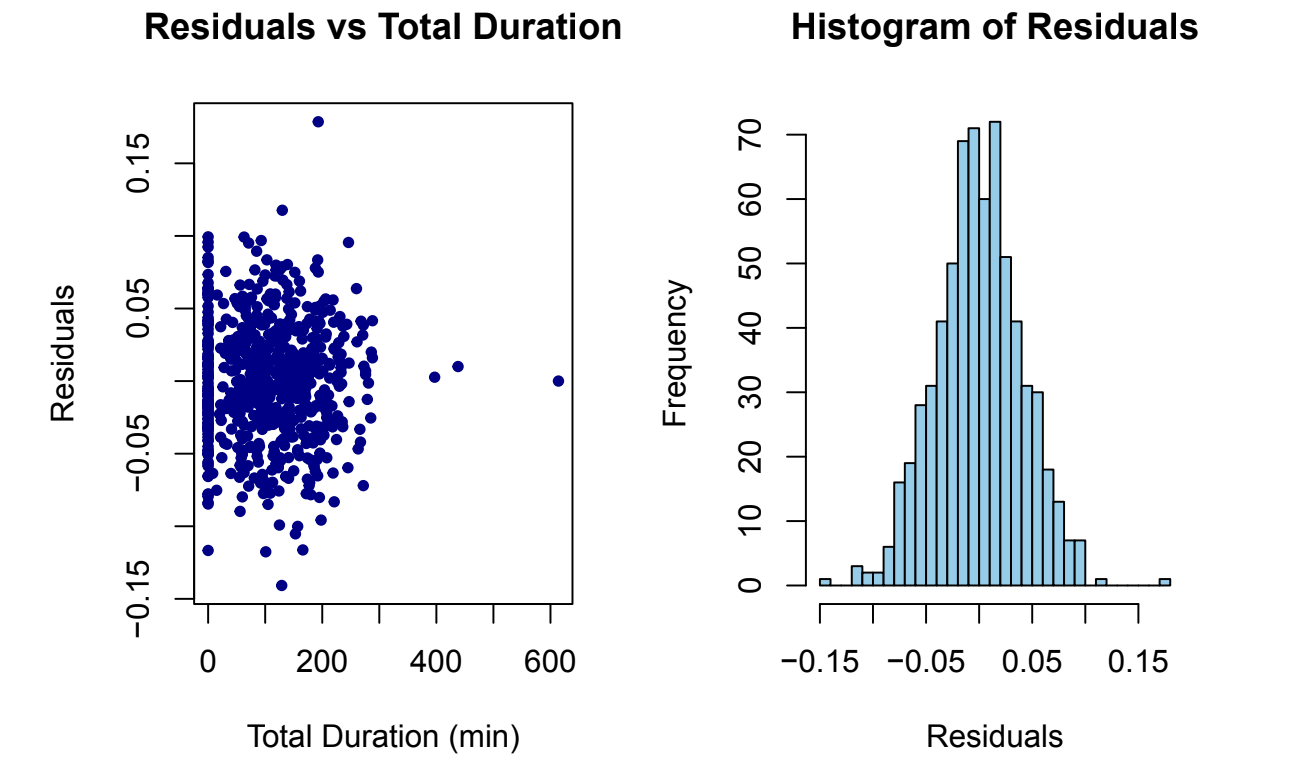
\includegraphics[width=0.6\textwidth]{images/pred_model_backward_plot2.png}
  \caption{Prediction: Residuals vs Fitted Values and Q-Q Plot of Residuals}
  \label{fig:residuals_fitted_qq}
\end{figure}


\end{document}
